%% LyX 2.3.7 created this file.  For more info, see http://www.lyx.org/.
%% Do not edit unless you really know what you are doing.
\documentclass[journal,article,submit,pdftex,moreauthors]{Definitions/mdpi}
\usepackage[utf8]{inputenc}
\usepackage{float}
\usepackage{url}
\usepackage{graphicx}

\makeatletter

%%%%%%%%%%%%%%%%%%%%%%%%%%%%%% LyX specific LaTeX commands.

\Title{Combining constructed artificial neural networks with parameter constraint
techniques to achieve better generalization properties}

\TitleCitation{Combining constructed artificial neural networks with parameter constraint
techniques to achieve better generalization properties}

\Author{Ioannis G. Tsoulos$^{1,*}$, Vasileios Charilogis$^{2}$, Dimitrios
Tsalikakis$^{3}$}

\AuthorNames{Ioannis G. Tsoulos, Vasileios Charilogis, Dimitrios Tsalikakis}

\AuthorCitation{Tsoulos, I.G.; Charilogis, V.; Tsalikakis D.}


\address{$^{1}$\quad{}Department of Informatics and Telecommunications,
University of Ioannina, Greece;itsoulos@uoi.gr\\
$^{2}$\quad{}Department of Informatics and Telecommunications, University
of Ioannina, Greece; v.charilog@uoi.gr\\
$^{3}\quad$Department of Engineering Informatics and Telecommunications,
University of Western Macedonia, 50100 Kozani, Greece; tsalikakis@gmail.com}


\corres{Correspondence: itsoulos@uoi.gr}


\abstract{A machine learning technology that has been used in a wide range
of everyday problems is the recently proposed technique of constructing
artificial neural networks with the assistance of Grammatical Evolution.
This technique was utilized in problems from the fields of physics,
chemistry, medicine, etc., in which it had excellent performance compared
to other machine learning models. A key feature of these machine learning
models is that they can both construct the structure of an artificial
neural network efficiently and identify optimal values of the parameters
of this network at the same time. However, in many cases the optimization
process can become trapped in local minima of the error function,
resulting in the construction of the artificial neural network not
being able to be completed satisfactorily, which will lead to poor
results in terms of test error. In this work, the combination of the
artificial neural network construction method with an adapted genetic
algorithm is proposed, which preserves the structure of the neural
network that has been constructed and, in addition, appropriately
adapts the parameters of the artificial neural network in order to
avoid overfitting problems. The proposed method was applied on a wide
series of datasets from real world problems that include classification
and regression problems and it was compared against traditional machine
learning models and the results are reported.}


\keyword{Grammatical Evolution; Genetic Programming; Neural networks; Local
Optimization}

\DeclareTextSymbolDefault{\textquotedbl}{T1}
%% Because html converters don't know tabularnewline
\providecommand{\tabularnewline}{\\}
\floatstyle{ruled}
\newfloat{algorithm}{tbp}{loa}
\providecommand{\algorithmname}{Algorithm}
\floatname{algorithm}{\protect\algorithmname}

%%%%%%%%%%%%%%%%%%%%%%%%%%%%%% Textclass specific LaTeX commands.
\newenvironment{lyxcode}
	{\par\begin{list}{}{
		\setlength{\rightmargin}{\leftmargin}
		\setlength{\listparindent}{0pt}% needed for AMS classes
		\raggedright
		\setlength{\itemsep}{0pt}
		\setlength{\parsep}{0pt}
		\normalfont\ttfamily}%
	 \item[]}
	{\end{list}}

%%%%%%%%%%%%%%%%%%%%%%%%%%%%%% User specified LaTeX commands.
%  LaTeX support: latex@mdpi.com 
%  For support, please attach all files needed for compiling as well as the log file, and specify your operating system, LaTeX version, and LaTeX editor.

%=================================================================


% For posting an early version of this manuscript as a preprint, you may use "preprints" as the journal and change "submit" to "accept". The document class line would be, e.g., \documentclass[preprints,article,accept,moreauthors,pdftex]{mdpi}. This is especially recommended for submission to arXiv, where line numbers should be removed before posting. For preprints.org, the editorial staff will make this change immediately prior to posting.

%--------------------
% Class Options:
%--------------------
%----------
% journal
%----------
% Choose between the following MDPI journals:
% acoustics, actuators, addictions, admsci, adolescents, aerospace, agriculture, agriengineering, agronomy, ai, algorithms, allergies, alloys, analytica, animals, antibiotics, antibodies, antioxidants, applbiosci, appliedchem, appliedmath, applmech, applmicrobiol, applnano, applsci, aquacj, architecture, arts, asc, asi, astronomy, atmosphere, atoms, audiolres, automation, axioms, bacteria, batteries, bdcc, behavsci, beverages, biochem, bioengineering, biologics, biology, biomass, biomechanics, biomed, biomedicines, biomedinformatics, biomimetics, biomolecules, biophysica, biosensors, biotech, birds, bloods, blsf, brainsci, breath, buildings, businesses, cancers, carbon, cardiogenetics, catalysts, cells, ceramics, challenges, chemengineering, chemistry, chemosensors, chemproc, children, chips, cimb, civileng, cleantechnol, climate, clinpract, clockssleep, cmd, coasts, coatings, colloids, colorants, commodities, compounds, computation, computers, condensedmatter, conservation, constrmater, cosmetics, covid, crops, cryptography, crystals, csmf, ctn, curroncol, currophthalmol, cyber, dairy, data, dentistry, dermato, dermatopathology, designs, diabetology, diagnostics, dietetics, digital, disabilities, diseases, diversity, dna, drones, dynamics, earth, ebj, ecologies, econometrics, economies, education, ejihpe, electricity, electrochem, electronicmat, electronics, encyclopedia, endocrines, energies, eng, engproc, ent, entomology, entropy, environments, environsciproc, epidemiologia, epigenomes, est, fermentation, fibers, fintech, fire, fishes, fluids, foods, forecasting, forensicsci, forests, foundations, fractalfract, fuels, futureinternet, futureparasites, futurepharmacol, futurephys, futuretransp, galaxies, games, gases, gastroent, gastrointestdisord, gels, genealogy, genes, geographies, geohazards, geomatics, geosciences, geotechnics, geriatrics, hazardousmatters, healthcare, hearts, hemato, heritage, highthroughput, histories, horticulturae, humanities, humans, hydrobiology, hydrogen, hydrology, hygiene, idr, ijerph, ijfs, ijgi, ijms, ijns, ijtm, ijtpp, immuno, informatics, information, infrastructures, inorganics, insects, instruments, inventions, iot, j, jal, jcdd, jcm, jcp, jcs, jdb, jeta, jfb, jfmk, jimaging, jintelligence, jlpea, jmmp, jmp, jmse, jne, jnt, jof, joitmc, jor, journalmedia, jox, jpm, jrfm, jsan, jtaer, jzbg, kidney, kidneydial, knowledge, land, languages, laws, life, liquids, literature, livers, logics, logistics, lubricants, lymphatics, machines, macromol, magnetism, magnetochemistry, make, marinedrugs, materials, materproc, mathematics, mca, measurements, medicina, medicines, medsci, membranes, merits, metabolites, metals, meteorology, methane, metrology, micro, microarrays, microbiolres, micromachines, microorganisms, microplastics, minerals, mining, modelling, molbank, molecules, mps, msf, mti, muscles, nanoenergyadv, nanomanufacturing, nanomaterials, ncrna, network, neuroglia, neurolint, neurosci, nitrogen, notspecified, nri, nursrep, nutraceuticals, nutrients, obesities, oceans, ohbm, onco, oncopathology, optics, oral, organics, organoids, osteology, oxygen, parasites, parasitologia, particles, pathogens, pathophysiology, pediatrrep, pharmaceuticals, pharmaceutics, pharmacoepidemiology, pharmacy, philosophies, photochem, photonics, phycology, physchem, physics, physiologia, plants, plasma, pollutants, polymers, polysaccharides, poultry, powders, preprints, proceedings, processes, prosthesis, proteomes, psf, psych, psychiatryint, psychoactives, publications, quantumrep, quaternary, qubs, radiation, reactions, recycling, regeneration, religions, remotesensing, reports, reprodmed, resources, rheumato, risks, robotics, ruminants, safety, sci, scipharm, seeds, sensors, separations, sexes, signals, sinusitis, skins, smartcities, sna, societies, socsci, software, soilsystems, solar, solids, sports, standards, stats, stresses, surfaces, surgeries, suschem, sustainability, symmetry, synbio, systems, taxonomy, technologies, telecom, test, textiles, thalassrep, thermo, tomography, tourismhosp, toxics, toxins, transplantology, transportation, traumacare, traumas, tropicalmed, universe, urbansci, uro, vaccines, vehicles, venereology, vetsci, vibration, viruses, vision, waste, water, wem, wevj, wind, women, world, youth, zoonoticdis 

%---------
% article
%---------
% The default type of manuscript is "article", but can be replaced by: 
% abstract, addendum, article, book, bookreview, briefreport, casereport, comment, commentary, communication, conferenceproceedings, correction, conferencereport, entry, expressionofconcern, extendedabstract, datadescriptor, editorial, essay, erratum, hypothesis, interestingimage, obituary, opinion, projectreport, reply, retraction, review, perspective, protocol, shortnote, studyprotocol, systematicreview, supfile, technicalnote, viewpoint, guidelines, registeredreport, tutorial
% supfile = supplementary materials

%----------
% submit
%----------
% The class option "submit" will be changed to "accept" by the Editorial Office when the paper is accepted. This will only make changes to the frontpage (e.g., the logo of the journal will get visible), the headings, and the copyright information. Also, line numbering will be removed. Journal info and pagination for accepted papers will also be assigned by the Editorial Office.

%------------------
% moreauthors
%------------------
% If there is only one author the class option oneauthor should be used. Otherwise use the class option moreauthors.

%---------
% pdftex
%---------
% The option pdftex is for use with pdfLaTeX. If eps figures are used, remove the option pdftex and use LaTeX and dvi2pdf.

%=================================================================
% MDPI internal commands - do not modify
\firstpage{1} 
 
\setcounter{page}{\@firstpage} 

\pubvolume{1}
\issuenum{1}
\articlenumber{0}
\pubyear{2024}
\copyrightyear{2024}
%\externaleditor{Academic Editor: Firstname Lastname} % For journal Automation, please change Academic Editor to "Communicated by"
\datereceived{}
\daterevised{ } % Comment out if no revised date
\dateaccepted{}
\datepublished{}
%\datecorrected{} % Corrected papers include a "Corrected: XXX" date in the original paper.
%\dateretracted{} % Corrected papers include a "Retracted: XXX" date in the original paper.
\hreflink{https://doi.org/} % If needed use \linebreak
%\doinum{}
%------------------------------------------------------------------
% The following line should be uncommented if the LaTeX file is uploaded to arXiv.org
%\pdfoutput=1

%=================================================================
% Add packages and commands here. The following packages are loaded in our class file: fontenc, inputenc, calc, indentfirst, fancyhdr, graphicx, epstopdf, lastpage, ifthen, lineno, float, amsmath, setspace, enumitem, mathpazo, booktabs, titlesec, etoolbox, tabto, xcolor, soul, multirow, microtype, tikz, totcount, changepage, attrib, upgreek, cleveref, amsthm, hyphenat, natbib, hyperref, footmisc, url, geometry, newfloat, caption

%=================================================================
%% Please use the following mathematics environments: Theorem, Lemma, Corollary, Proposition, Characterization, Property, Problem, Example, ExamplesandDefinitions, Hypothesis, Remark, Definition, Notation, Assumption
%% For proofs, please use the proof environment (the amsthm package is loaded by the MDPI class).

%=================================================================
% The fields PACS, MSC, and JEL may be left empty or commented out if not applicable
%\PACS{J0101}
%\MSC{}
%\JEL{}

%%%%%%%%%%%%%%%%%%%%%%%%%%%%%%%%%%%%%%%%%%
% Only for the journal Diversity
%\LSID{\url{http://}}

%%%%%%%%%%%%%%%%%%%%%%%%%%%%%%%%%%%%%%%%%%
% Only for the journal Applied Sciences:
%\featuredapplication{Authors are encouraged to provide a concise description of the specific application or a potential application of the work. This section is not mandatory.}
%%%%%%%%%%%%%%%%%%%%%%%%%%%%%%%%%%%%%%%%%%

%%%%%%%%%%%%%%%%%%%%%%%%%%%%%%%%%%%%%%%%%%
% Only for the journal Data:
%\dataset{DOI number or link to the deposited data set in cases where the data set is published or set to be published separately. If the data set is submitted and will be published as a supplement to this paper in the journal Data, this field will be filled by the editors of the journal. In this case, please make sure to submit the data set as a supplement when entering your manuscript into our manuscript editorial system.}

%\datasetlicense{license under which the data set is made available (CC0, CC-BY, CC-BY-SA, CC-BY-NC, etc.)}

%%%%%%%%%%%%%%%%%%%%%%%%%%%%%%%%%%%%%%%%%%
% Only for the journal Toxins
%\keycontribution{The breakthroughs or highlights of the manuscript. Authors can write one or two sentences to describe the most important part of the paper.}

%%%%%%%%%%%%%%%%%%%%%%%%%%%%%%%%%%%%%%%%%%
% Only for the journal Encyclopedia
%\encyclopediadef{Instead of the abstract}
%\entrylink{The Link to this entry published on the encyclopedia platform.}
%%%%%%%%%%%%%%%%%%%%%%%%%%%%%%%%%%%%%%%%%%

%%%%%%%%%%%%%%%%%%%%%%%%%%%%%%%%%%%%%%%%%%
% Only for the journal Advances in Respiratory Medicine
%\addhighlights{yes}
%\renewcommand{\addhighlights}{%

%\noindent This is an obligatory section in “Advances in Respiratory Medicine”, whose goal is to increase the discoverability and readability of the article via search engines and other scholars. Highlights should not be a copy of the abstract, but a simple text allowing the reader to quickly and simplified find out what the article is about and what can be cited from it. Each of these parts should be devoted up to 2~bullet points.\vspace{3pt}\\
%\textbf{What are the main findings?}
% \begin{itemize}[labelsep=2.5mm,topsep=-3pt]
% \item First bullet.
% \item Second bullet.
% \end{itemize}\vspace{3pt}
%\textbf{What is the implication of the main finding?}
% \begin{itemize}[labelsep=2.5mm,topsep=-3pt]
% \item First bullet.
% \item Second bullet.
% \end{itemize}
%}
%%%%%%%%%%%%%%%%%%%%%%%%%%%%%%%%%%%%%%%%%%

\makeatother

\begin{document}
\maketitle

\section{Introduction}

A basic machine learning technique with a wide range of applications
in data classification and regression problems is artificial neural
networks \citep{nn1,nn2}. Artificial neural networks are parametric
machine learning model, in which learning is achieved by effectively
adjusting their parameters through any optimization technique. The
optimization procedure minimizes the so - called training error of
an artificial neural network and it is defined as: 
\begin{equation}
E\left(N\left(\overrightarrow{x},\overrightarrow{w}\right)\right)=\sum_{i=1}^{M}\left(N\left(\overrightarrow{x}_{i},\overrightarrow{w}\right)-y_{i}\right)^{2}\label{eq:eq1}
\end{equation}
In this equation the function $N\left(\overrightarrow{x},\overrightarrow{w}\right)$
represents the artificial neural network which is applied on a vector
$\overrightarrow{x}$ and the vector $\overrightarrow{w}$ denotes
the parameter vector of the neural network. The set $\left(\overrightarrow{x_{i}},y_{i}\right),\ i=1,...,M$
represents the training set of the objective problem and the values
$y_{i}$ are the expected outputs for each pattern $\overrightarrow{x_{i}}$. 

Artificial neural networks have been applied in a wide series of problems
appeared in real - world problems, such as image processing \citep{nn_image},
time series forecasting \citep{nn_timeseries}, credit card analysis
\citep{nn_credit}, problems derived from physics \citep{nnphysics1,nnphysics2}
etc. Due to the widespread use of these machine learning models, a
number of techniques have been proposed to minimize the equation \ref{eq:eq1},
such as the Back Propagation algorithm \citep{bpnn1,bpnn2}, the RPROP
algorithm \citep{rpropnn-1,rpropnn-2}, the ADAM optimization method
\citep{nn_adam} etc. Also, recently a series of more advanced global
optimization methods have been proposed to tackle the training of
neural networks. Among them one can locate the incorporation of Genetic
Algorithms \citep{geneticnn1}, the usage of the Particle Swarm Optimization
(PSO) method \citep{psonn}, the Simulated Annealing method \citep{nn_siman},
the Differential Evolution technique \citep{weight_de1}, the Artificial
Bee Colony (ABC) method \citep{nn_abc} etc. Furthermore, Sexton et
al suggested the usage of the tabu search algorithm for optimal neural
network training \citep{tabunn}, Zhang et al proposed a hybrid algorithm
that incorporated the PSO method and the Back Propagation algorithm
to efficient train artificial neural networks \citep{nn_hybrid}.
Also, recently Zhao et al introduced a new Cascaded Forward Algorithm
to train artificial neural networks \citep{nn_cascade}. Furthermore,
due to the rapid spread of the use of parallel computing techniques,
a series of computational techniques have emerged that exploit parallel
computing structures for faster training of artificial neural networks
\citep{nn_gpu1,nn_gpu2}.

However, the above techniques, although extremely effective, nevertheless
have a number of problems such as, for example, trapping in local
minima of the error function or the phenomenon of overifitting, where
the artificial neural network exhibits reduced performance when applied
to data that was not present during the training process. The overfitting
problem has been studied by many researchers that have proposed a
series of methods to handle this problem, such as weight sharing \citep{nnsharing1,nnsharing2},
pruning \citep{nnprunning1,nnprunning2}, early stopping \citep{nnearly1,nnearly2},
weight decaying \citep{nndecay1,nndecay2} etc. Also, many researchers
propose as a solution to the above problem the dynamic creation of
the architecture of artificial neural networks using programming techniques.
For example the Genetic Algorithms were proposed to create dynamically
the optimal architecture of neural networks \citep{nn_arch1,nn_arch2}
or the PSO method \citep{nn_arch3}.

A method that was proposed relatively recently and it is based on
Grammatical Evolution \citep{ge1}, dynamically identifies both the
optimal architecture of artificial neural networks and the optimal
values of its parameters \citep{nnc}. This method has been applied
in a series of problems in the recent literature, such as problems
presented in chemistry \citep{nnc_amide1}, identification of the
solution of differential equations \citep{nnc_de}, medical problems
\citep{nnc_feas}, problems related to education \citep{nnc_student},
autism screening \citep{nnc_autism} etc. A key advantage of this
technique is that it can isolate from the initial features of the
problem those that are most important in training the model, thus
significantly reducing the required number of parameters that need
to be identified.

However, the method of constructing artificial neural networks can
easily get trapped in local minima of the training error since it
does not have any technique to avoid them. Furthermore, although the
method can get quite close to a minimum of the training error, it
often does not reach it since there is no technique in the method
to train the generated parameters. In this technique, it is proposed
to enhance the original method of constructing artificial neural networks
by periodically applying a modified genetic algorithm to randomly
selected chromosomes of Grammatical Evolution. This modified genetic
algorithm preserves the architecture created by the Grammatical Evolution
method and effectively locates the parameters of the artificial neural
network by reducing the training error. In addition, the proposed
genetic algorithm through appropriate penalty factors imposed on the
fitness function prevents the artificial neural network from overfitting.

The remaining of this article is organized as follows: in section
\ref{sec:Method-description} the proposed method and the accompanied
genetic algorithm are introduced, in section \ref{sec:Results} the
experimental datasets and the series of experiments conducted are
listed and discussed thoroughly and final in section \ref{sec:Conclusions}
some conclusions are discussed.

\section{Method description\label{sec:Method-description}}

This section provides a details description of the original neural
network construction method and continuous with the proposed genetic
algorithm and concludes with the overall algorithm.

\subsection{The neural construction method \label{subsec:The-neural-construction}}

The neural construction method utilizes the technique of Grammatical
Evolution to produce artificial neural networks. Grammatical Evolution
is an evolutionary process where the chromosomes are vectors of positive
integers. These integers represent rules from a Backs - Naur form
(BNF) grammar \citep{bnf1} of the target language.\textbf{ }The method
was incorporated in various cases, such as data fitting\textbf{ }\citep{ge_program1,ge_program2},
composition of music \citep{ge_music}, video games \citep{ge_pacman,ge_supermario},
energy problems \citep{ge_energy}, cryptography \citep{ge_crypt},
economics \citep{ge_trading} etc. Any BNF grammar is defined as a
set\textbf{ $G=\left(N,T,S,P\right)$ }where the letters have the
following definitions:
\begin{itemize}
\item The set $N$ represents the non - terminal symbols of the grammar.
\item The set $T$ contains the terminal symbols of the grammar. 
\item The start symbol of the grammar is denoted as $S$.
\item The production rules of the grammar are enclosed in the set $P$
\end{itemize}
The Grammatical Evolution production procedure initiates from the
starting symbol $S$ and following a series of steps, the method creates
valid programs by replacing non-terminal symbols with the right hand
of the selected production rule. The selection scheme has as:
\begin{itemize}
\item \textbf{Read} the next element V from the chromosome that is being
processed.
\item \textbf{Select} the next production rule following the equation:Rule
= V mod $N_{R}$. The symbol $N_{R}$ represents the total number
of production rules for the under processing non -- terminal symbol. 
\end{itemize}
The process of producing valid programs through the Grammatical Evolution
method is depicted graphically in Figure \ref{fig:geProcess}.

\begin{figure}[H]
\begin{centering}

\includegraphics[scale=0.5]{GEFC}
\par\end{centering}
\caption{The Grammatical Evolution process used to produce valid programs.\label{fig:geProcess}}

\end{figure}
The grammar used for the neural construction procedure is shown in
Figure \ref{fig:nncGrammar}. The numbers shown in parentheses are
the increasing numbers of the production rules for each non - terminal
symbol. The constant $d$ denotes the number of features in every
pattern of the input dataset.

\begin{figure}[H]
\begin{lyxcode}
S:=\textless Sigval\textgreater ~~~~~~~~~~~~~~~~~~~~~~~~~~(0)

\textless Sigval\textgreater ::=\textless Node\textgreater ~~~~~~~~~~~~~~~~~~~~(0)

~~~~~~~~~~~\textbar ~\textless Node\textgreater ~+~\textless Sigval\textgreater ~~~~~~~(1)

\textless Node\textgreater ::=\textless Number\textgreater{*}sig(\textless Sum\textgreater +\textless Number\textgreater )~(0)

\textless Sum\textgreater ::=~\textless Number\textgreater{*}\textless Xlist\textgreater ~~~~~~~~~~~~(0)

~~~~~~~~~~~\textbar ~~~~\textless Sum\textgreater +\textless Sum\textgreater ~~~~~~~~~~~(1)

\textless Xlist\textgreater ::=~x1~~~~~~~~(0)

~~~~~~~~~~~~~\textbar ~~~~x2~~(1)

~~~~~~~~~~~~~..............

~~~~~~~~~~~~~\textbar ~~~~xd~~(d-1)

\textless Number\textgreater ::=~(\textless Dlist\textgreater .\textless Dlist\textgreater )~~~~~~~~(0)

~~~~~~~~~~~~~\textbar ~~~~(-\textless Dlist\textgreater .\textless Dlist\textgreater )~(1)

\textless Dlist\textgreater ::=~\textless Digit\textgreater ~~~~~~~~~~~~(0)

~~~~~~~~~~~~~\textbar ~\textless Digit\textgreater\textless Dlist\textgreater ~(1)

\textless Digit\textgreater ::=~0~~~~~~(0)

~~~~~~~~~~~~~\textbar ~~1~(1)

~~~~~~~~~~~~~...........

~~~~~~~~~~~~~\textbar ~~9~(9)
\end{lyxcode}
\caption{The proposed grammar for the construction of artificial neural networks
through Grammatical Evolution.\label{fig:nncGrammar}}
\end{figure}
The used grammar produces artificial neural networks with the following
form:

\begin{equation}
N\left(\overrightarrow{x},\overrightarrow{w}\right)=\sum_{i=1}^{H}w_{(d+2)i-(d+1)}\sigma\left(\sum_{j=1}^{d}x_{j}w_{(d+2)i-(d+1)+j}+w_{(d+2)i}\right)\label{eq:nn}
\end{equation}
The term $H$ stands for the number of processing units (weights)
of the neural network. The The function $\sigma(x)$ represents the
sigmoid function.\textbf{ }The total number of parameters for this
network are computed through the following equation:
\begin{equation}
n=\left(d+2\right)H
\end{equation}
For example the following form:
\begin{equation}
N(x)=1.9\mbox{sig}\left(10.5x_{1}+3.2x_{3}+1.4\right)+2.1\mbox{sig}\left(2.2x_{2}-3.3x_{3}+3.2\right)
\end{equation}
denotes a produced neural network for a problem with 3 inputs $\left(x_{1},x_{2},x_{3}\right)$
and the number of processing nodes is $H=2$. The neural network produced
can be shown graphically in Figure \ref{fig:nnExample}.

\begin{figure}[H]
\begin{centering}
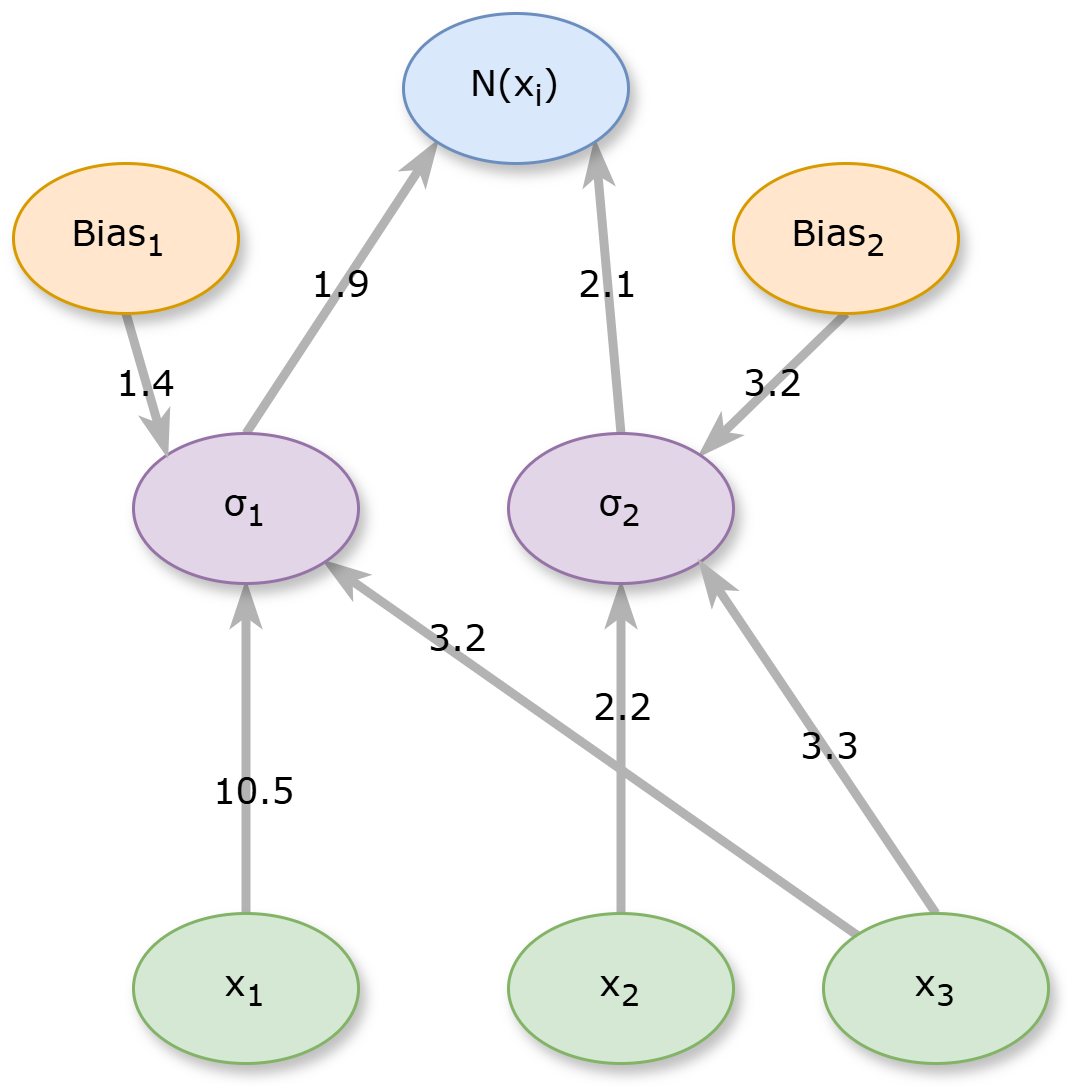
\includegraphics[scale=0.75]{example_diagram}
\par\end{centering}
\caption{An example of a produced neural network.\label{fig:nnExample}}

\end{figure}


\subsection{The used genetic algorithm \label{subsec:The-used-genetic}}

In the original method of constructing artificial neural networks,
it is proposed in this work to introduce the concept of local search,
through the periodic application of a genetic algorithm which should
maintain the structure of the neural network constructed by the original
method. Additionally, a second goal of this genetic algorithm should
be to avoid the problem of overfitting that could arise from simply
applying a local optimization method to the previous artificial neural
network. For the first goal of the modified genetic algorithm consider
the example neural network shown before:
\begin{equation}
N(x)=1.9\mbox{sig}\left(10.5x_{1}+3.2x_{3}+1.4\right)+2.1\mbox{sig}\left(2.2x_{2}-3.3x_{3}+3.2\right)
\end{equation}
The weight vector $\overrightarrow{w}$ for this neural network would
be 
\begin{equation}
\overrightarrow{w}=\left[1.9,10.5,0.0,3.2,1.4,2.1,0.0,2.2,-3.3,3.2\right]\label{eq:exampleNN}
\end{equation}
In order to protect the structure of this artificial neural network,
the modified genetic algorithm should allow changes in the parameters
of this network within a value interval, which can be considered to
be the pair of vectors $\left[\overrightarrow{L,}\overrightarrow{R}\right]$.
The elements for the vector $\overrightarrow{L}$ are defined as 
\begin{equation}
L_{i}=-F\times\left|w_{i}\right|,\ i=1,\ldots,n\label{eq:createL}
\end{equation}
where $F$ is positive number with $F>1$. Likewise the right bound
for the parameters $\overrightarrow{R}$ is defined from the following
equation:
\begin{equation}
R_{i}=F\times\left|w_{i}\right|,i=1,\ldots,n\label{eq:createR}
\end{equation}
For the example weight vector of equation \ref{eq:exampleNN} and
for $F=2$ the following vectors are used:
\[
\begin{array}{ccc}
L & = & \left[-3.8,-21.0,0.0,-6.4,-2.8,-4.2,0.0,-4.4,-6.6,-6.4\right]\\
R & = & \left[\ \ \ 3.8,\ \ \ 21.0,0.0,\ \ \ 6.4,\ \ \ \ 2.8,\ \ \ \ 4.2,0.0,\ \ \ 4.4,\ \ \ 6.6,\ \ \ \ 6.4\right]
\end{array}
\]
The modified genetic algorithm should also prevent the artificial
neural networks it trains from the phenomenon of overfitting, which
would lead to poor results on the test dataset. For this reason a
quantity derived from the publication of Anastasopoulos et al. \citep{nnt_bound}
is utilized here. The sigmoid function, that is used as the activation
function of neural networks is defined as:
\begin{equation}
\sigma(x)=\frac{1}{1+\exp(-x)}
\end{equation}
A plot for this function is shown in Figure \ref{fig:plotsigma}.

\begin{figure}[H]
\begin{centering}
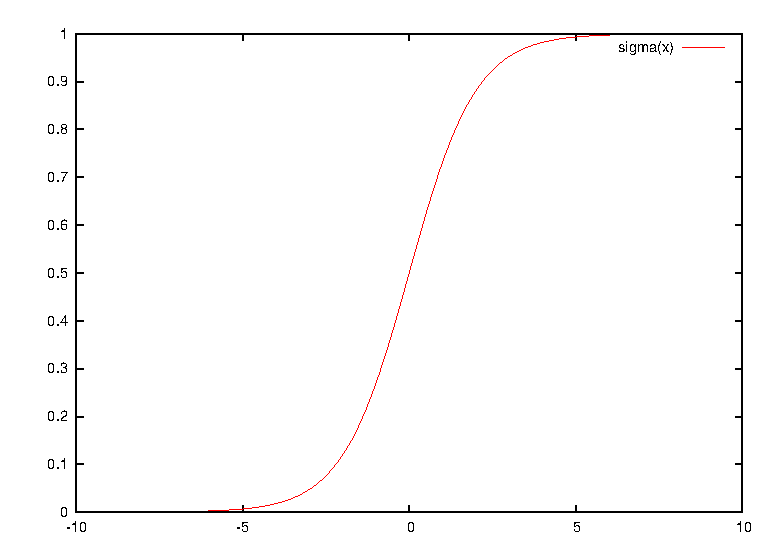
\includegraphics[scale=0.75]{sig}
\par\end{centering}
\caption{Plot of the sigmoid function $\sigma(x)$.\label{fig:plotsigma}}

\end{figure}
As is clear from the equation and the figure, as the value of the
parameter x increases, the function tends very quickly to 1. On the
other hand, the function will take values very close to 0 as the parameter
x decreases. This means that the function very quickly loses the generalizing
abilities it has and therefore large changes in the value of the parameter
x will not cause proportional variations in the value of the sigmoid
function. Therefore, the quantity $B\left(N\left(\overrightarrow{x},\overrightarrow{w}\right),a\right)$
was introduced in that paper to measure this effect. This quantity
is calculated through the process of Algorithm \ref{alg:CalculationBound}.

\begin{algorithm}[H]
\caption{The algorithm used to calculate the bounding quantity for neural network
$N(x,w)$.\label{alg:CalculationBound}}

\textbf{function} $\mbox{evalB}\left(N\left(\overrightarrow{x},\overrightarrow{w}\right),a\right)$
\begin{enumerate}
\item \textbf{Inputs}: The Neural network $N\left(\overrightarrow{x},\overrightarrow{w}\right)$
and the double precision value $a,\ a>1$.
\item \textbf{Set} $s=0$
\item \textbf{For} $i=1..H$ \textbf{Do}
\begin{enumerate}
\item \textbf{For} $j=1..M$ \textbf{Do}
\begin{enumerate}
\item \textbf{Calculate} $v=\sum_{kT=1}^{d}w_{(d+2)i-(d+i)+k}x_{jk}+w_{(d+2)i}$
\item \textbf{If} $\left|v\right|>a$ \textbf{set} $s=s+1$
\end{enumerate}
\item \textbf{EndFor}
\end{enumerate}
\item \textbf{EndFor}
\item \textbf{Return} $\frac{s}{H\star M}$
\end{enumerate}
\textbf{End Function}
\end{algorithm}
The overall proposed modified genetic algorithm is shown in Algorithm
\ref{alg:The-modified-Genetic}.

\begin{algorithm}[H]
\caption{The modified Genetic Algorithm.\label{alg:The-modified-Genetic}}

\textbf{Function} $\mbox{mGA}\left(\overrightarrow{L},\overrightarrow{R,}a,\lambda\right)$
\begin{enumerate}
\item \textbf{Input}s: The bound vectors $\overrightarrow{L,}\overrightarrow{R}$
and the bounding factor $a$ and $\lambda$ a positive value with
$\lambda>1$.
\item \textbf{Set} as $N_{K}$the number of allowed generations and as $N_{G}$
the number of used chromosomes.
\item \textbf{Set} as $p_{S}$ the selection rate and as $p_{M}$ the mutation
rate.
\item \textbf{Initialize} $N_{G}$ chromosomes inside the bounding boxes
$\overrightarrow{L,}\overrightarrow{R}$.
\item \textbf{Set} $k=0$, the generation number.
\item \textbf{For} $i=1,\ldots,N_{G}$\label{enu:For}
\begin{enumerate}
\item \textbf{Obtain} the corresponding neural network $N_{i}\left(\overrightarrow{x},\overrightarrow{g_{i}}\right)$
for the chromosome $g_{i}$.
\item \textbf{Set} $e_{i}=\sum_{j=1}^{M}\left(N_{i}\left(\overrightarrow{x}_{j},\overrightarrow{w_{i}}\right)-y_{j}\right)^{2}$
\item \textbf{Set} $B_{i}=\mbox{eval}\left(N_{i}\left(\overrightarrow{x},\overrightarrow{g_{i}}\right),a\right)$
using the algorithm \ref{alg:CalculationBound}.
\item \textbf{Set} $f_{i}=e_{i}\times\left(1+\lambda B_{i}^{2}\right)$
as the fitness value of chromosome $g_{i}$
\end{enumerate}
\item \textbf{End For}
\item \textbf{Select} the best $\left(1-p_{s}\right)\times N_{G}$ chromosomes,
that will be copied intact to the next generation. The remaining will
be substituted by individuals produced by crossover and mutation.
\item \textbf{Set} $k=k+1$
\item \textbf{If} $k\le N_{K}$ \textbf{goto} step \ref{enu:For}.
\end{enumerate}
\textbf{End function}
\end{algorithm}


\subsection{The overall algorithm}

The overall algorithm uses the procedures presented previously to
achieve greater accuracy in calculations as well as to avoid overfitting
phenomena. The steps of the overall algorithm have as follows:
\begin{enumerate}
\item \textbf{Initialization}.
\begin{enumerate}
\item \textbf{Set} as $N_{C}$ the number of chromosomes for the Grammatical
Evolution procedure and as $N_{G}$ the maximum number of allowed
generations.
\item \textbf{Set} as $p_{S}$ the selection rate and as $p_{M}$ the mutation
rate.
\item \textbf{Let} $N_{I}$ be the number of chromosomes to which the modified
genetic algorithm will be periodically applied. 
\item \textbf{Let} $N_{T}$ be the number of generations that will pass
before applying the modified genetic algorithm to randomly selected
chromosomes.
\item \textbf{Set} the weight factor $F$ with $F>1$.
\item \textbf{Set} the values $N_{K},\ a,\ \lambda$ used in the modified
genetic algorithm.
\item \textbf{Initialize} randomly the $N_{C}$ chromosomes as sets of randomly
selected integers.
\item \textbf{Set} the generation number $k=0$ 
\end{enumerate}
\item \textbf{Fitness Calculation}.
\begin{enumerate}
\item \textbf{For} $i=1,\ldots,N_{C}$ \textbf{do}
\begin{enumerate}
\item \textbf{Obtain} the chromosome $g_{i}$
\item \textbf{Create} the corresponding neural network $N_{i}\left(\overrightarrow{x},\overrightarrow{w}\right)$
using Grammatical Evolution.
\item \textbf{Set} the fitness value $f_{i}=\sum_{j=1}^{M}\left(N_{i}\left(\overrightarrow{x}_{j},\overrightarrow{w}\right)-y_{j}\right)^{2}$
\end{enumerate}
\item \textbf{End For}
\end{enumerate}
\item \textbf{Genetic Operations}.
\begin{enumerate}
\item \textbf{Select} the best $\left(1-p_{s}\right)\times N_{G}$ chromosomes,
that will be copied intact to the next generation. 
\item \textbf{Create} $p_{S}N$ chromosomes using one - point crossover.
For every couple $\left(c_{1},c_{2}\right)$ of produced offsprings
two distinct chromosomes are selected from the current population
using tournament selection. An example of the one - point crossover
procedure is shown graphically in Figure \ref{fig:onePoint}.
\item For every chromosome and for each element select a random number $r\le1$.
Alter the current element when $r\le p_{M}$
\end{enumerate}
\item \textbf{Local search.}
\begin{enumerate}
\item \textbf{If} $k\ \mbox{mod}\ N_{T}=0$ \textbf{then}
\begin{enumerate}
\item \textbf{Set} $S=\left\{ g_{r_{1}},g_{r_{2}},\ldots,g_{r_{N_{I}}}\right\} $
a group of $N_{I}$ randomly selected chromosomes from the genetic
population.
\item \textbf{For} every member $g\in S$ \textbf{do}
\begin{enumerate}
\item \textbf{Obtain} the corresponding neural network $N_{g}\left(\overrightarrow{x},\overrightarrow{w}\right)$
for the chromosome $g$.
\item \textbf{Create} the left bound vector $\overrightarrow{L_{g}}$ and
the right bound vector $\overrightarrow{R_{g}}$ for $g$ using the
equations \ref{eq:createL},\ref{eq:createR} respectively.
\item \textbf{Set} $g=\mbox{mga}\left(\overrightarrow{L_{g}},\overrightarrow{R_{g},}a,\lambda\right)$
using the steps of algorithm \ref{alg:The-modified-Genetic}.
\end{enumerate}
\item \textbf{End For}
\end{enumerate}
\item \textbf{Endif}
\end{enumerate}
\item \textbf{Termination Check}.
\begin{enumerate}
\item \textbf{Set} $k=k+1$
\item \textbf{If} $k\le N_{G}$ goto \textbf{Fitness Calculation}.
\end{enumerate}
\item \textbf{Application to the test set}.
\begin{enumerate}
\item \textbf{Obtain} the chromosome $g^{*}$ with the lowest fitness value
and create through Grammatical Evolution the corresponding neural
network $N^{*}\left(\overrightarrow{x},\overrightarrow{w}\right)$
\item \textbf{Apply} the neural network $N^{*}\left(\overrightarrow{x},\overrightarrow{w}\right)$
and report the corresponding error value.
\end{enumerate}
%
\end{enumerate}
\begin{figure}[H]
\begin{centering}
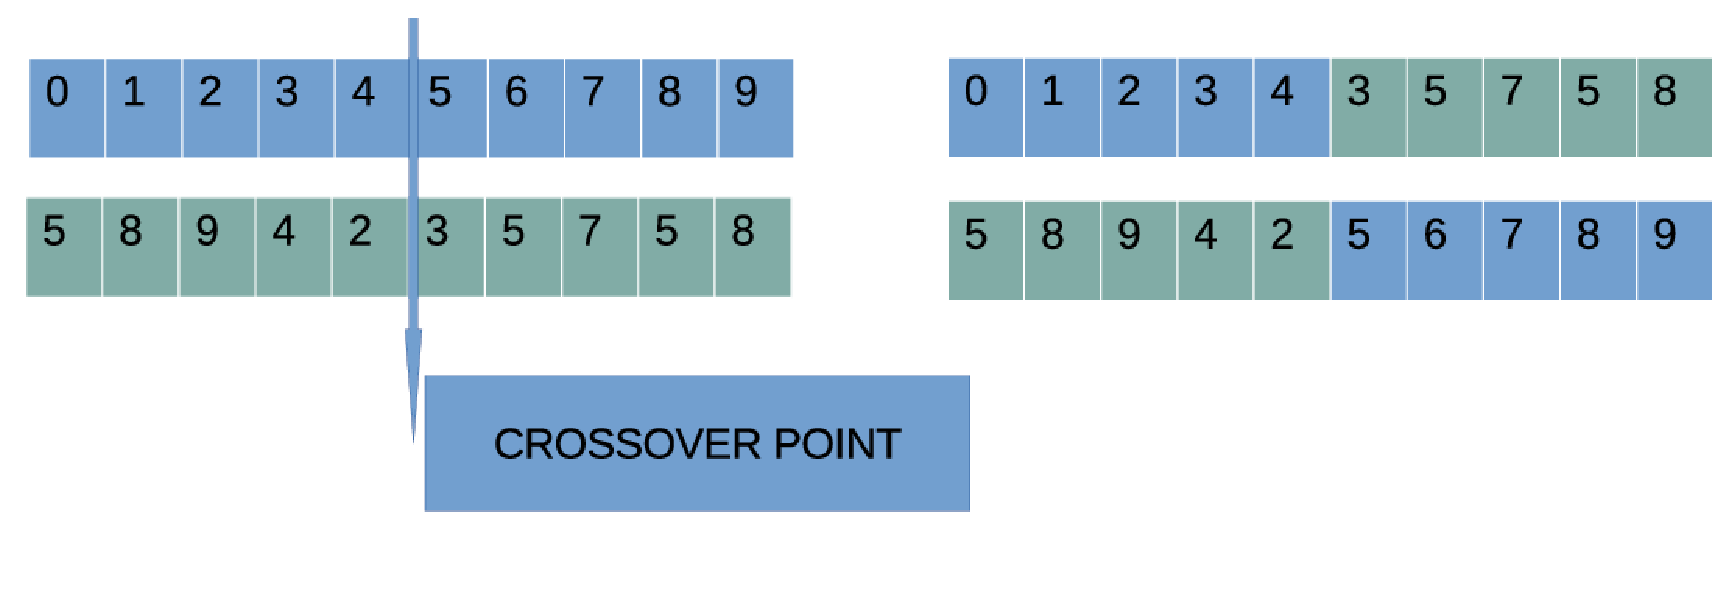
\includegraphics[scale=0.5]{onepoint_crossover}
\par\end{centering}
\caption{An example of the one - point crossover procedure.\label{fig:onePoint}}

\end{figure}


\section{Experimental results\label{sec:Results}}

The validation of the proposed method was performed using a wide series
of classification and regression datasets, available from various
sources from the Internet. These datasets were downloaded from:
\begin{enumerate}
\item The UCI database, \url{https://archive.ics.uci.edu/}(accessed on
22 January 2025)\citep{uci}
\item The Keel website, \url{https://sci2s.ugr.es/keel/datasets.php}(accessed
on 22 January 2025)\citep{Keel}.
\item The Statlib URL \url{https://lib.stat.cmu.edu/datasets/index}(accessed
on 22 January 2025). 
\end{enumerate}

\subsection{Experimental datasets }

The following datasets were utilized in the conducted experiments:
\begin{enumerate}
\item \textbf{Appendictis} which is a medical dataset \citep{appendicitis}. 
\item \textbf{Alcohol}, which is dataset regarding alcohol consumption \citep{alcohol}. 
\item \textbf{Australian}, which is a dataset produced from various bank
transactions \citep{australian}.
\item \textbf{Balance} dataset \citep{balance}, produced from various psychological
experiments.
\item \textbf{Cleveland}, a medical dataset which was discussed in a series
of papers \citep{cleveland1,cleveland2}. 
\item \textbf{Circular} dataset, which is an artificial dataset.
\item \textbf{Dermatology}, a medical dataset for dermatology problems \citep{dermatology}.
\item \textbf{Ecoli}, which is related to protein problems \citep{ecoli}.
\item \textbf{Glass} dataset, that contains measurements from glass component
analysis. 
\item \textbf{Haberman}, a medical dataset related to breast cancer.
\item \textbf{Hayes-roth} dataset \citep{hayes-roth}.
\item \textbf{Heart}, which is a dataset related to heart diseases \citep{heart}.
\item \textbf{HeartAttack}, which is a medical dataset for the detection
of heart diseases
\item \textbf{Housevotes}, a dataset which is related to the Congressional
voting in USA \citep{housevotes}.
\item \textbf{Ionosphere}, a dataset that contains measurements from the
ionosphere \citep{ion1,ion2}.
\item \textbf{Liverdisorder}, a medical dataset that was studied thoroughly
in a series of papers\citep{liver,liver1}.
\item \textbf{Lymography} \citep{lymography}.
\item \textbf{Mammographic}, which is a medical dataset used for the prediction
of breast cancer \citep{mammographic}.
\item \textbf{Parkinsons}, which is a medical dataset used for the detection
of Parkinson's disease \citep{parkinsons1,parkinsons2}.
\item \textbf{Pima}, which is a medical dataset for the detection of diabetes\citep{pima}.
\item \textbf{Phoneme}, a dataset that contains sound measurements.
\item \textbf{Popfailures}, a dataset related to experiments regarding climate
\citep{popfailures}.
\item \textbf{Regions2}, a medical dataset applied to liver problems \citep{regions2}.
\item \textbf{Saheart}, which is a medical dataset concerning heart diseases\citep{saheart}.
\item \textbf{Segment} dataset \citep{segment}.
\item \textbf{Statheart}, a medical dataset related to heart diseases.
\item \textbf{Spiral}, an artificial dataset with two classes.
\item \textbf{Student}, which is a dataset regarding experiments in schools
\citep{student}.
\item \textbf{Transfusion}, which is a medical dataset \citep{transfusion}.
\item \textbf{Wdbc}, which is a medical dataset regarding breast cancer
\citep{wdbc1,wdbc2}.
\item \textbf{Wine}, a dataset regarding measurements about the quality
of wines \citep{wine1,wine2}.
\item \textbf{EEG}, which is dataset regardingEEG recordings \citep{eeg1,eeg2}.
From this dataset the following cases were used: Z\_F\_S, ZO\_NF\_S,
ZONF\_S and Z\_O\_N\_F\_S.
\item \textbf{Zoo}, which is a dataset regarding animal classification \citep{zoo}
.
\end{enumerate}
Moreover a series of regression datasets was adopted in the conducted
experiments. The list with the regression datasets has as follows:
\begin{enumerate}
\item \textbf{Abalone}, which is a dataset about the age of abalones \citep{abalone}.
\item \textbf{Airfoil}, a dataset founded in NASA \citep{airfoil}.
\item \textbf{Auto}, a dataset related to the consumption of fuels from
cars.
\item \textbf{BK}, which is used to predict the points scored in basketball
games. 
\item \textbf{BL}, a dataset that contains measurements from electricity
experiments.
\item \textbf{Baseball}, which is a dataset used to predict the income of
baseball players.
\item \textbf{Concrete}, which is a civil engineering dataset \citep{concrete}.
\item \textbf{DEE}, a dataset that is used to predict the price of electricity.
\item \textbf{Friedman}, which is an artificial dataset\citep{friedman}.
\item \textbf{FY, }which is a dataset regarding the longevity of fruit flies. 
\item \textbf{HO}, a dataset located in the STATLIB repository.
\item \textbf{Housing}, regarding the price of houses \citep{housing}.
\item \textbf{Laser}, which contains measurements from various physics experiments.
\item \textbf{LW}, a dataset regarding the weight of babes.
\item \textbf{Mortgage}, a dataset that contains measurements from the economy
of USA.
\item \textbf{PL} dataset, located in the STALIB repository.
\item \textbf{Plastic}, a dataset regarding problems occurred with the pressure
on plastics.
\item \textbf{Quake}, a dataset regarding the measurements of earthquakes.
\item \textbf{SN}, a dataset related to trellising and pruning.
\item \textbf{Stock}, which is a dataset regarding stocks.
\item \textbf{Treasury}, a dataset that contains measurements from the economy
of USA.
\end{enumerate}

\subsection{Experiments}

The software used in the experiment was coded in C++ with the assistance
of the freely available Optimus environment, that can be downloaded
from \url{https://github.com/itsoulos/GlobalOptimus/}( accessed on
23 January 2025 ). Every experiments was conducted 30 times and each
time different seed for the random generator was used. The experiments
were validated using the ten - fold cross validation technique. The
average classification error, as measured in the corresponding test
set was reported for the classification datasets. This error is calculated
through the following formula:
\begin{equation}
E_{C}\left(N\left(\overrightarrow{x},\overrightarrow{w}\right)\right)=100\times\frac{\sum_{i=1}^{N}\left(\mbox{class}\left(N\left(\overrightarrow{x_{i}},\overrightarrow{w}\right)\right)-y_{i}\right)}{N}
\end{equation}
Here the test set $T$ is a set $T=\left(x_{i},y_{i}\right),\ i=1,\ldots,N$.
Likewise, the average regression error is reported for the regression
datasets. This error can be obtained using the following equation:
\begin{equation}
E_{R}\left(N\left(\overrightarrow{x},\overrightarrow{w}\right)\right)=\frac{\sum_{i=1}^{N}\left(N\left(\overrightarrow{x_{i}},\overrightarrow{w}\right)-y_{i}\right)^{2}}{N}
\end{equation}
The experiments were executed on\textbf{ }an AMD Ryzen 5950X with
128GB of RAM and the used operating system was Debian Linux. The values
for the parameters of the proposed method are shown in Table \ref{tab:expValues}. 

\begin{table}[H]
\begin{centering}
\begin{tabular}{|c|c|c|}
\hline 
PARAMETER & MEANING & VALUE\tabularnewline
\hline 
\hline 
$N_{C}$ & Chromosomes & 500\tabularnewline
\hline 
$N_{G}$ & Maximum number of generations & 500\tabularnewline
\hline 
$N_{K}$ & Number of generations for the modified Genetic Algorithm & 50\tabularnewline
\hline 
$p_{S}$ & Selection rate & 0.1\tabularnewline
\hline 
$p_{M}$ & Mutation rate & 0.05\tabularnewline
\hline 
$N_{T}$ & Generations before local search & 20\tabularnewline
\hline 
$N_{I}$ & Chromosomes participating in local search & 20\tabularnewline
\hline 
$a$ & Bounding factor & 10.0\tabularnewline
\hline 
$F$ & Scale factor for the margins & 2.0\tabularnewline
\hline 
$\lambda$ & Value used for penalties & 100.0\tabularnewline
\hline 
\end{tabular}
\par\end{centering}
\caption{The values for the parameters of the proposed method.\label{tab:expValues}}
\end{table}

In the following tables that describe the experimental results the
following notation is used:
\begin{enumerate}
\item The column DATASET represents the used dataset.
\item The column ADAM represents the incorporation of the ADAM optimization
method \citep{nn_adam} to train a neural network with $H=10$ processing
nodes.
\item The column BFGS stands for the usage of a BFGS variant of Powell \citep{powell}
to train an artificial neural network with $H=10$ processing nodes.
\item The column GENETIC represents the incorporation of a Genetic Algorithm
with the same parameter set as provided in Table \ref{tab:expValues}
to train a neural network with $H=10$ processing nodes.
\item The column RBF describes the experimental results obtained by the
application of a Radial Basis Function (RBF) network \citep{rbf1,rbf2}
with $H=10$ hidden nodes.
\item The column NNC stands for the usage of the original neural construction
method.
\item The column PROPOSED denotes the usage of the proposed method.
\item The row AVERAGE represents the average classification or regression
error for all datasets in the corresponding table.
\end{enumerate}
In Table \ref{tab:expClass}, the performance of different machine
learning algorithms on various classification datasets is shown, as
measured by error rates. Each column represents a specific machine
learning model, while each row corresponds to a dataset and the error
rate associated with each algorithm for that particular dataset. The
last row of the table presents the average error rates for each algorithm,
providing an overall view of their performance. The analysis begins
with the observation that the \textquotedbl PROPOSED\textquotedbl{}
model demonstrates the lowest average error rate (21.18\%) compared
to all other models. This indicates that, overall, it delivers the
best performance, producing the most accurate results across this
set of data. In many datasets, such as APPENDICITIS, BALANCE, and
ZOO, the \textquotedbl PROPOSED\textquotedbl{} model achieves the
lowest error rates, specifically 14.30\%, 7.84\%, and 6.60\%, respectively,
showcasing its strong performance in these cases. However, it is not
consistently the best, as in some datasets, like MAMMOGRAPHIC and
CIRCULAR, other models exhibit slightly lower error rates.The \textquotedbl GENETIC\textquotedbl{}
model records the highest average error rate, at 28.25\%, which suggests
its overall performance is the weakest across this dataset collection.
However, it is noted that in certain datasets, such as CIRCULAR and
HOUSEVOTES, the \textquotedbl GENETIC\textquotedbl{} model performs
relatively well with error rates of 5.99\% and 6.62\%, respectively,
which are comparable to those of the more effective models. This indicates
that its performance may depend on the specific characteristics of
each dataset. Another noteworthy algorithm is \textquotedbl BFGS,\textquotedbl{}
which has an average error rate of 35.71\%. While its performance
is not consistently strong, significant deviations are observed in
certain datasets, such as DERMATOLOGY and SEGMENT. For instance, in
DERMATOLOGY, it exhibits an error rate of 52.92\%, whereas the \textquotedbl PROPOSED\textquotedbl{}
model achieves 20.54\%, highlighting the substantial sensitivity of
\textquotedbl BFGS\textquotedbl{} to the peculiarities of this dataset.
In datasets with substantial variability in error rates, such as AUSTRALIAN
and STATHEART, significant differentiation between algorithms is observed.
In AUSTRALIAN, the \textquotedbl PROPOSED\textquotedbl{} model achieves
the lowest error rate of 14.55\%, while other algorithms exhibit error
rates ranging from 32.21\% to 38.13\%. This difference underscores
the superiority of the \textquotedbl PROPOSED\textquotedbl{} model
in datasets that pose specific challenges to other algorithms. Similarly,
in STATHEART, the \textquotedbl PROPOSED\textquotedbl{} model achieves
one of the lowest error rates (17.93\%), whereas other algorithms,
such as \textquotedbl GENETIC,\textquotedbl{} show rates as high
as 27.25\%.

\begin{table}[H]
\caption{Experimental results using a variety of machine learning methods for
the classification datasets.\label{tab:expClass}}

\centering{}%
\begin{tabular}{|c|c|c|c|c|c|c|}
\hline 
DATASET & ADAM & BFGS & GENETIC & RBF & NNC & PROPOSED\tabularnewline
\hline 
\hline 
APPENDICITIS & 16.50\% & 18.00\% & 24.40\% & 12.23\% & 14.40\% & 14.30\%\tabularnewline
\hline 
ALCOHOL & 57.78\% & 41.50\% & 39.57\% & 49.32\% & 37.72\% & 35.60\%\tabularnewline
\hline 
AUSTRALIAN & 35.65\% & 38.13\% & 32.21\% & 34.89\% & 14.46\% & 14.55\%\tabularnewline
\hline 
BALANCE & 12.27\% & 8.64\% & 8.97\% & 33.53\% & 23.65\% & 7.84\%\tabularnewline
\hline 
CLEVELAND & 67.55\% & 77.55\% & 51.60\% & 67.10\% & 50.93\% & 46.41\%\tabularnewline
\hline 
CIRCULAR & 19.95\% & 6.08\% & 5.99\% & 5.98\% & 12.66\% & 6.92\%\tabularnewline
\hline 
DERMATOLOGY & 26.14\% & 52.92\% & 30.58\% & 62.34\% & 21.54\% & 20.54\%\tabularnewline
\hline 
ECOLI & 64.43\% & 69.52\% & 54.67\% & 59.48\% & 49.88\% & 48.82\%\tabularnewline
\hline 
GLASS & 61.38\% & 54.67\% & 52.86\% & 50.46\% & 56.09\% & 53.52\%\tabularnewline
\hline 
HABERMAN & 29.00\% & 29.34\% & 28.66\% & 25.10\% & 27.53\% & 26.80\%\tabularnewline
\hline 
HAYES-ROTH & 59.70\% & 37.33\% & 56.18\% & 64.36\% & 33.69\% & 31.00\%\tabularnewline
\hline 
HEART & 38.53\% & 39.44\% & 28.34\% & 31.20\% & 15.67\% & 15.45\%\tabularnewline
\hline 
HEARTATTACK & 45.55\% & 46.67\% & 29.03\% & 29.00\% & 20.87\% & 21.77\%\tabularnewline
\hline 
HOUSEVOTES & 7.48\% & 7.13\% & 6.62\% & 6.13\% & 3.17\% & 3.78\%\tabularnewline
\hline 
IONOSPHERE & 16.64\% & 15.29\% & 15.14\% & 16.22\% & 11.29\% & 11.94\%\tabularnewline
\hline 
LIVERDISORDER & 41.53\% & 42.59\% & 31.11\% & 30.84\% & 32.35\% & 31.32\%\tabularnewline
\hline 
LYMOGRAPHY & 39.79\% & 35.43\% & 28.42\% & 25.50\% & 25.29\% & 23.72\%\tabularnewline
\hline 
MAMMOGRAPHIC & 46.25\% & 17.24\% & 19.88\% & 21.38\% & 17.62\% & 16.74\%\tabularnewline
\hline 
PARKINSONS & 24.06\% & 27.58\% & 18.05\% & 17.41\% & 12.74\% & 12.63\%\tabularnewline
\hline 
PHONEME & 29.43\% & 15.58\% & 15.55\% & 23.32\% & 22.50\% & 21.52\%\tabularnewline
\hline 
PIMA & 34.85\% & 35.59\% & 32.19\% & 25.78\% & 28.07\% & 23.34\%\tabularnewline
\hline 
POPFAILURES & 5.18\% & 5.24\% & 5.94\% & 7.04\% & 6.98\% & 5.72\%\tabularnewline
\hline 
REGIONS2 & 29.85\% & 36.28\% & 29.39\% & 38.29\% & 26.18\% & 23.81\%\tabularnewline
\hline 
SAHEART & 34.04\% & 37.48\% & 34.86\% & 32.19\% & 29.80\% & 28.04\%\tabularnewline
\hline 
SEGMENT & 49.75\% & 68.97\% & 57.72\% & 59.68\% & 53.50\% & 48.20\%\tabularnewline
\hline 
SPIRAL & 47.67\% & 47.99\% & 48.66\% & 44.87\% & 48.01\% & 44.95\%\tabularnewline
\hline 
STATHEART & 44.04\% & 39.65\% & 27.25\% & 31.36\% & 18.08\% & 17.93\%\tabularnewline
\hline 
STUDENT & 5.13\% & 7.14\% & 5.61\% & 5.49\% & 6.70\% & 4.05\%\tabularnewline
\hline 
TRANSFUSION & 25.68\% & 25.84\% & 24.87\% & 26.41\% & 25.77\% & 23.16\%\tabularnewline
\hline 
WDBC & 35.35\% & 29.91\% & 8.56\% & 7.27\% & 7.36\% & 4.95\%\tabularnewline
\hline 
WINE & 29.40\% & 59.71\% & 19.20\% & 31.41\% & 13.59\% & 9.94\%\tabularnewline
\hline 
Z\_F\_S & 47.81\% & 39.37\% & 10.73\% & 13.16\% & 14.53\% & 7.97\%\tabularnewline
\hline 
Z\_O\_N\_F\_S & 78.79\% & 65.67\% & 64.81\% & 48.70\% & 48.62\% & 39.28\%\tabularnewline
\hline 
ZO\_NF\_S & 47.43\% & 43.04\% & 21.54\% & 9.02\% & 13.54\% & 6.94\%\tabularnewline
\hline 
ZONF\_S & 11.99\% & 15.62\% & 4.36\% & 4.03\% & 2.64\% & 2.60\%\tabularnewline
\hline 
ZOO & 14.13\% & 10.70\% & 9.50\% & 21.93\% & 8.70\% & 6.60\%\tabularnewline
\hline 
\textbf{AVERAGE} & \textbf{36.45\%} & \textbf{35.71\%} & \textbf{28.25\%} & \textbf{30.73\%} & \textbf{24.79\%} & \textbf{21.18\%}\tabularnewline
\hline 
\end{tabular}
\end{table}

The table \ref{tab:expRegression} presents the performance of various
machine learning models on regression datasets, as measured by absolute
error values. Each column represents a specific model, while each
row corresponds to a dataset and the absolute error value associated
with each algorithm for that dataset. The last row provides the average
error values for each algorithm, offering a general view of their
overall performance. The analysis shows that the \textquotedbl PROPOSED\textquotedbl{}
model achieves the lowest average error value (4.28) among all the
algorithms, indicating its superior overall performance in terms of
accuracy. Across multiple datasets, the \textquotedbl PROPOSED\textquotedbl{}
model consistently achieves the smallest error values, such as in
datasets like BL (0.001), MORTGAGE (0.023), and TREASURY (0.068).
These results highlight its effectiveness across various regression
problems. However, it is notable that in some datasets, such as FY
(0.043) and HOUSING (15.47), the \textquotedbl PROPOSED\textquotedbl{}
model does not have the lowest error values, though its performance
remains competitive. On the other hand, the \textquotedbl BFGS\textquotedbl{}
model records the highest average error value (30.29), reflecting
its generally weaker performance across the datasets. Its errors are
significantly higher in certain datasets, such as BASEBALL (119.63)
and STOCK (302.43), indicating challenges in addressing regression
tasks effectively in these cases. Despite this, \textquotedbl BFGS\textquotedbl{}
shows competitive performance in a few instances, such as in the AIRFOIL
dataset, where it achieves an error value of 0.003, close to that
of the \textquotedbl PROPOSED\textquotedbl{} model. The \textquotedbl GENETIC\textquotedbl{}
model has an average error value of 9.31, placing it among the mid-performing
models in this analysis. It performs relatively well in datasets like
MORTGAGE (2.41) and TREASURY (2.93), but struggles in others, such
as BASEBALL (103.6) and PLASTIC (2.791). These results indicate variability
in its performance depending on the dataset characteristics. The \textquotedbl ADAM\textquotedbl{}
model, with an average error value of 22.46, shows moderate performance
overall. It has strong results in some datasets, such as AIRFOIL (0.005)
and CONCRETE (0.078), but performs poorly in others, such as STOCK
(180.89) and BASEBALL (77.9). This suggests that \textquotedbl ADAM\textquotedbl{}
is sensitive to dataset-specific features and may not generalize well
across all cases. The \textquotedbl RBF\textquotedbl{} model achieves
an average error value of 10.02, demonstrating moderately good performance
across the datasets. It performs particularly well in datasets like
MORTGAGE (1.45) and LASER (0.03). However, it faces challenges in
datasets such as BASEBALL (93.02) and STOCK (12.23), where its error
values are notably higher. The \textquotedbl NNC\textquotedbl{} model
has an average error value of 6.29, placing it as a strong performer,
second only to the \textquotedbl PROPOSED\textquotedbl{} model in
this analysis. It shows competitive results across many datasets,
such as PL (0.047) and HO (0.015), but it is slightly outperformed
by \textquotedbl PROPOSED\textquotedbl{} in most cases, including
critical datasets like BL and TREASURY. Overall, the analysis reveals
the \textquotedbl PROPOSED\textquotedbl{} model's superiority in
minimizing absolute error across diverse regression datasets, as reflected
by its lowest average error. The results also underscore the variability
in performance among the other algorithms, suggesting that certain
models may perform better in specific contexts but lack consistent
efficacy across all datasets.

\begin{table}[H]
\caption{Experimental results using a variety of machine learning methods on
the regression datasets.\label{tab:expRegression}}

\centering{}%
\begin{tabular}{|c|c|c|c|c|c|c|}
\hline 
DATASET & ADAM & BFGS & GENETIC & RBF & NNC & PROPOSED\tabularnewline
\hline 
\hline 
ABALONE & 4.30 & 5.69 & 7.17 & 7.37 & 5.08 & 4.47\tabularnewline
\hline 
AIRFOIL & 0.005 & 0.003 & 0.003 & 0.27 & 0.004 & 0.002\tabularnewline
\hline 
AUTO & 70.84 & 60.97 & 12.18 & 17.87 & 17.13 & 9.09\tabularnewline
\hline 
BK & 0.0252 & 0.28 & 0.027 & 0.02 & 0.10 & 0.023\tabularnewline
\hline 
BL & 0.622 & 2.55 & 5.74 & 0.013 & 1.19 & 0.001\tabularnewline
\hline 
BASEBALL & 77.90 & 119.63 & 103.60 & 93.02 & 61.57 & 48.13\tabularnewline
\hline 
CONCRETE & 0.078 & 0.066 & 0.0099 & 0.011 & 0.008 & 0.005\tabularnewline
\hline 
DEE & 0.63 & 2.36 & 1.013 & 0.17 & 0.26 & 0.22\tabularnewline
\hline 
FRIEDMAN & 22.90 & 1.263 & 1.249 & 7.23 & 6.29 & 5.34\tabularnewline
\hline 
FY & 0.038 & 0.19 & 0.65 & 0.041 & 0.11 & 0.043\tabularnewline
\hline 
HO & 0.035 & 0.62 & 2.78 & 0.03 & 0.015 & 0.016\tabularnewline
\hline 
HOUSING & 80.99 & 97.38 & 43.26 & 57.68 & 25.47 & 15.47\tabularnewline
\hline 
LASER & 0.03 & 0.015 & 0.59 & 0.03 & 0.025 & 0.0049\tabularnewline
\hline 
LW & 0.028 & 2.98 & 1.90 & 0.03 & 0.011 & 0.011\tabularnewline
\hline 
MORTGAGE & 9.24 & 8.23 & 2.41 & 1.45 & 0.30 & 0.023\tabularnewline
\hline 
PL & 0.117 & 0.29 & 0.29 & 2.118 & 0.047 & 0.029\tabularnewline
\hline 
PLASTIC & 11.71 & 20.32 & 2.791 & 8.62 & 4.20 & 2.17\tabularnewline
\hline 
QUAKE & 0.07 & 0.42 & 0.04 & 0.07 & 0.96 & 0.036\tabularnewline
\hline 
SN & 0.026 & 0.40 & 2.95 & 0.027 & 0.026 & 0.024\tabularnewline
\hline 
STOCK & 180.89 & 302.43 & 3.88 & 12.23 & 8.92 & 4.69\tabularnewline
\hline 
TREASURY & 11.16 & 9.91 & 2.93 & 2.02 & 0.43 & 0.068\tabularnewline
\hline 
\textbf{AVERAGE} & \textbf{22.46} & \textbf{30.29} & \textbf{9.31} & \textbf{10.02} & \textbf{6.29} & \textbf{4.28}\tabularnewline
\hline 
\end{tabular}
\end{table}

In Figure \ref{fig:statClass}, the comparison of the proposed machine
learning model (PROPOSED) with other models on classification datasets
was conducted using a script in the R programming language, which
evaluated the p-value to assess the statistical significance of performance
differences. The p-value serves as a measure of the likelihood that
observed results are due to random variation rather than genuine differences
between the models. p-values below the commonly accepted threshold
of 0.05 indicate that the differences are statistically significant
and not due to random chance. The comparison between PROPOSED and
the ADAM model yielded a p-value of 1.9e-07, which is extremely low.
This indicates that the performance difference between the two models
is highly significant, rejecting the possibility that the superior
performance of PROPOSED is due to random variability. This result
highlights the clear advantage of PROPOSED over ADAM. In the case
of PROPOSED versus BFGS, the p-value was 1.1e-08, even smaller than
the comparison with ADAM. This extremely small p-value further underscores
that PROPOSED significantly outperforms BFGS, demonstrating that the
performance gap is exceptionally strong and statistically meaningful.
For the comparison of PROPOSED with GENETIC, the p-value was 6.9e-08.
Although this value is slightly higher than the previous ones, it
is still extraordinarily low, indicating that PROPOSED's performance
is clearly superior. This reinforces the consistency of PROPOSED when
compared to models relying on genetic algorithms. The p-value for
the comparison of PROPOSED with RBF was 1.9e-07, similar in magnitude
to the comparison with ADAM. This consistency indicates that the superiority
of PROPOSED over RBF is statistically significant, showcasing the
proposed model's robust performance against a model with a different
architecture. Finally, the comparison of PROPOSED with NNC produced
a p-value of 4.3e-08. This very low value demonstrates the strong
superiority of PROPOSED over a neural network classifier (NNC), further
emphasizing the general observation that the proposed model performs
better than the others, regardless of the specific technique employed
by each competing model. Overall, the exceptionally low p-values for
all comparisons provide evidence of the statistically significant
superiority of PROPOSED compared to the other models. The results
highlight that the performance of the proposed model is not only better
but also consistently superior, with differences that are robust and
highly reliable from a statistical perspective.

\begin{figure}[H]
\begin{centering}
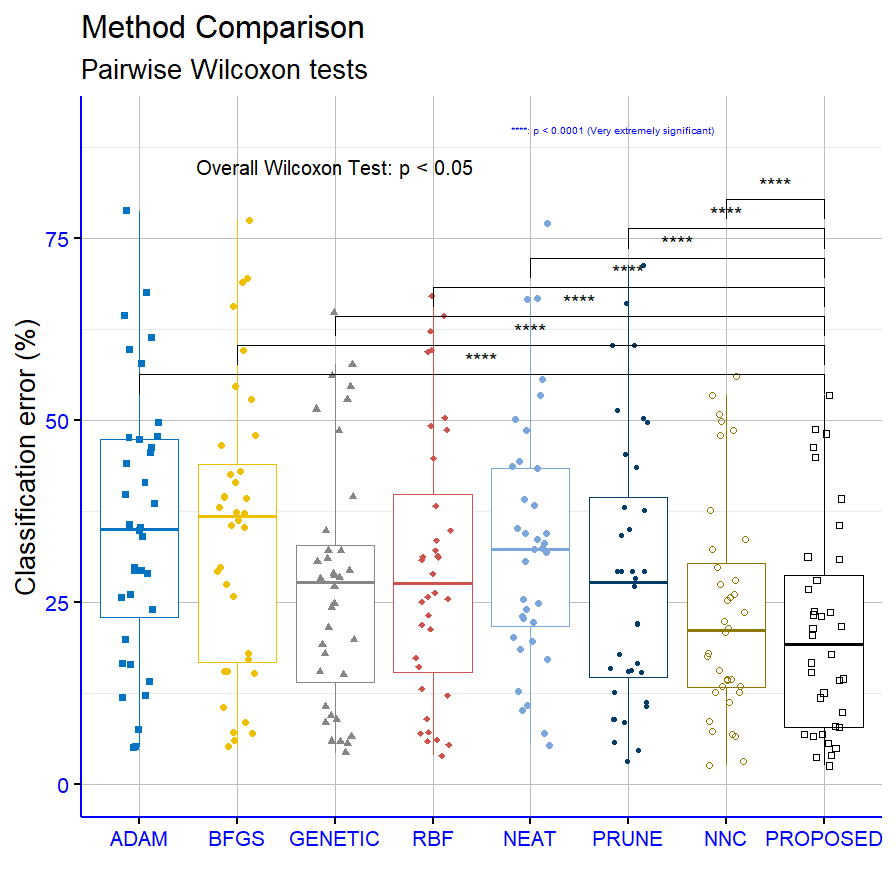
\includegraphics[scale=0.5]{new1}
\par\end{centering}
\caption{Statistical comparison of the machine learning models for the classification
datasets.\label{fig:statClass}}

\end{figure}
The comparison of the proposed machine learning model (PROPOSED) with
other models Figure \ref{fig:statRegression} on regression datasets
was conducted using statistical analysis to determine the p-values,
which measure the significance of performance differences between
the models. A low p-value indicates that the observed differences
are statistically significant and unlikely to have occurred by chance.
The results reveal a consistent and robust superiority of PROPOSED
over the other models. When comparing PROPOSED with ADAM, the p-value
was 0.00013. This low value indicates a statistically significant
difference in performance, confirming that the observed superiority
of PROPOSED is unlikely to be due to random variation. In the case
of BFGS, the p-value was even lower at 9.5e-07. This extremely small
value strongly supports the conclusion that PROPOSED significantly
outperforms BFGS, underscoring its robustness and reliability. The
comparison of PROPOSED with GENETIC yielded a p-value of 0.0001. This
result reaffirms the statistical significance of the performance gap
between the two models, highlighting PROPOSED’s consistent advantage
over GENETIC. For NEAT, the p-value was 0.0014, which, while slightly
higher than the previous values, is still well below the threshold
of 0.05. This demonstrates a statistically significant difference
in favor of PROPOSED, confirming its superior performance even when
compared to this specific algorithm. The comparison with RBF resulted
in a p-value of 0.00042. This low value further solidifies the observation
that PROPOSED consistently performs better than RBF, providing evidence
of its strong adaptability and reliability across various regression
datasets. Finally, the comparison with PRUNE yielded a p-value of
0.00011, which, like the others, is extremely low. This demonstrates
that the performance differences between PROPOSED and PRUNE are statistically
significant, further validating the superiority of the proposed model.
Overall, the low p-values across all comparisons provide compelling
evidence of the statistical significance of the performance advantages
of PROPOSED over the other models in regression tasks. These results
emphasize the consistency and reliability of the proposed model in
delivering superior results across a wide range of regression datasets.

\begin{figure}[H]
\begin{centering}
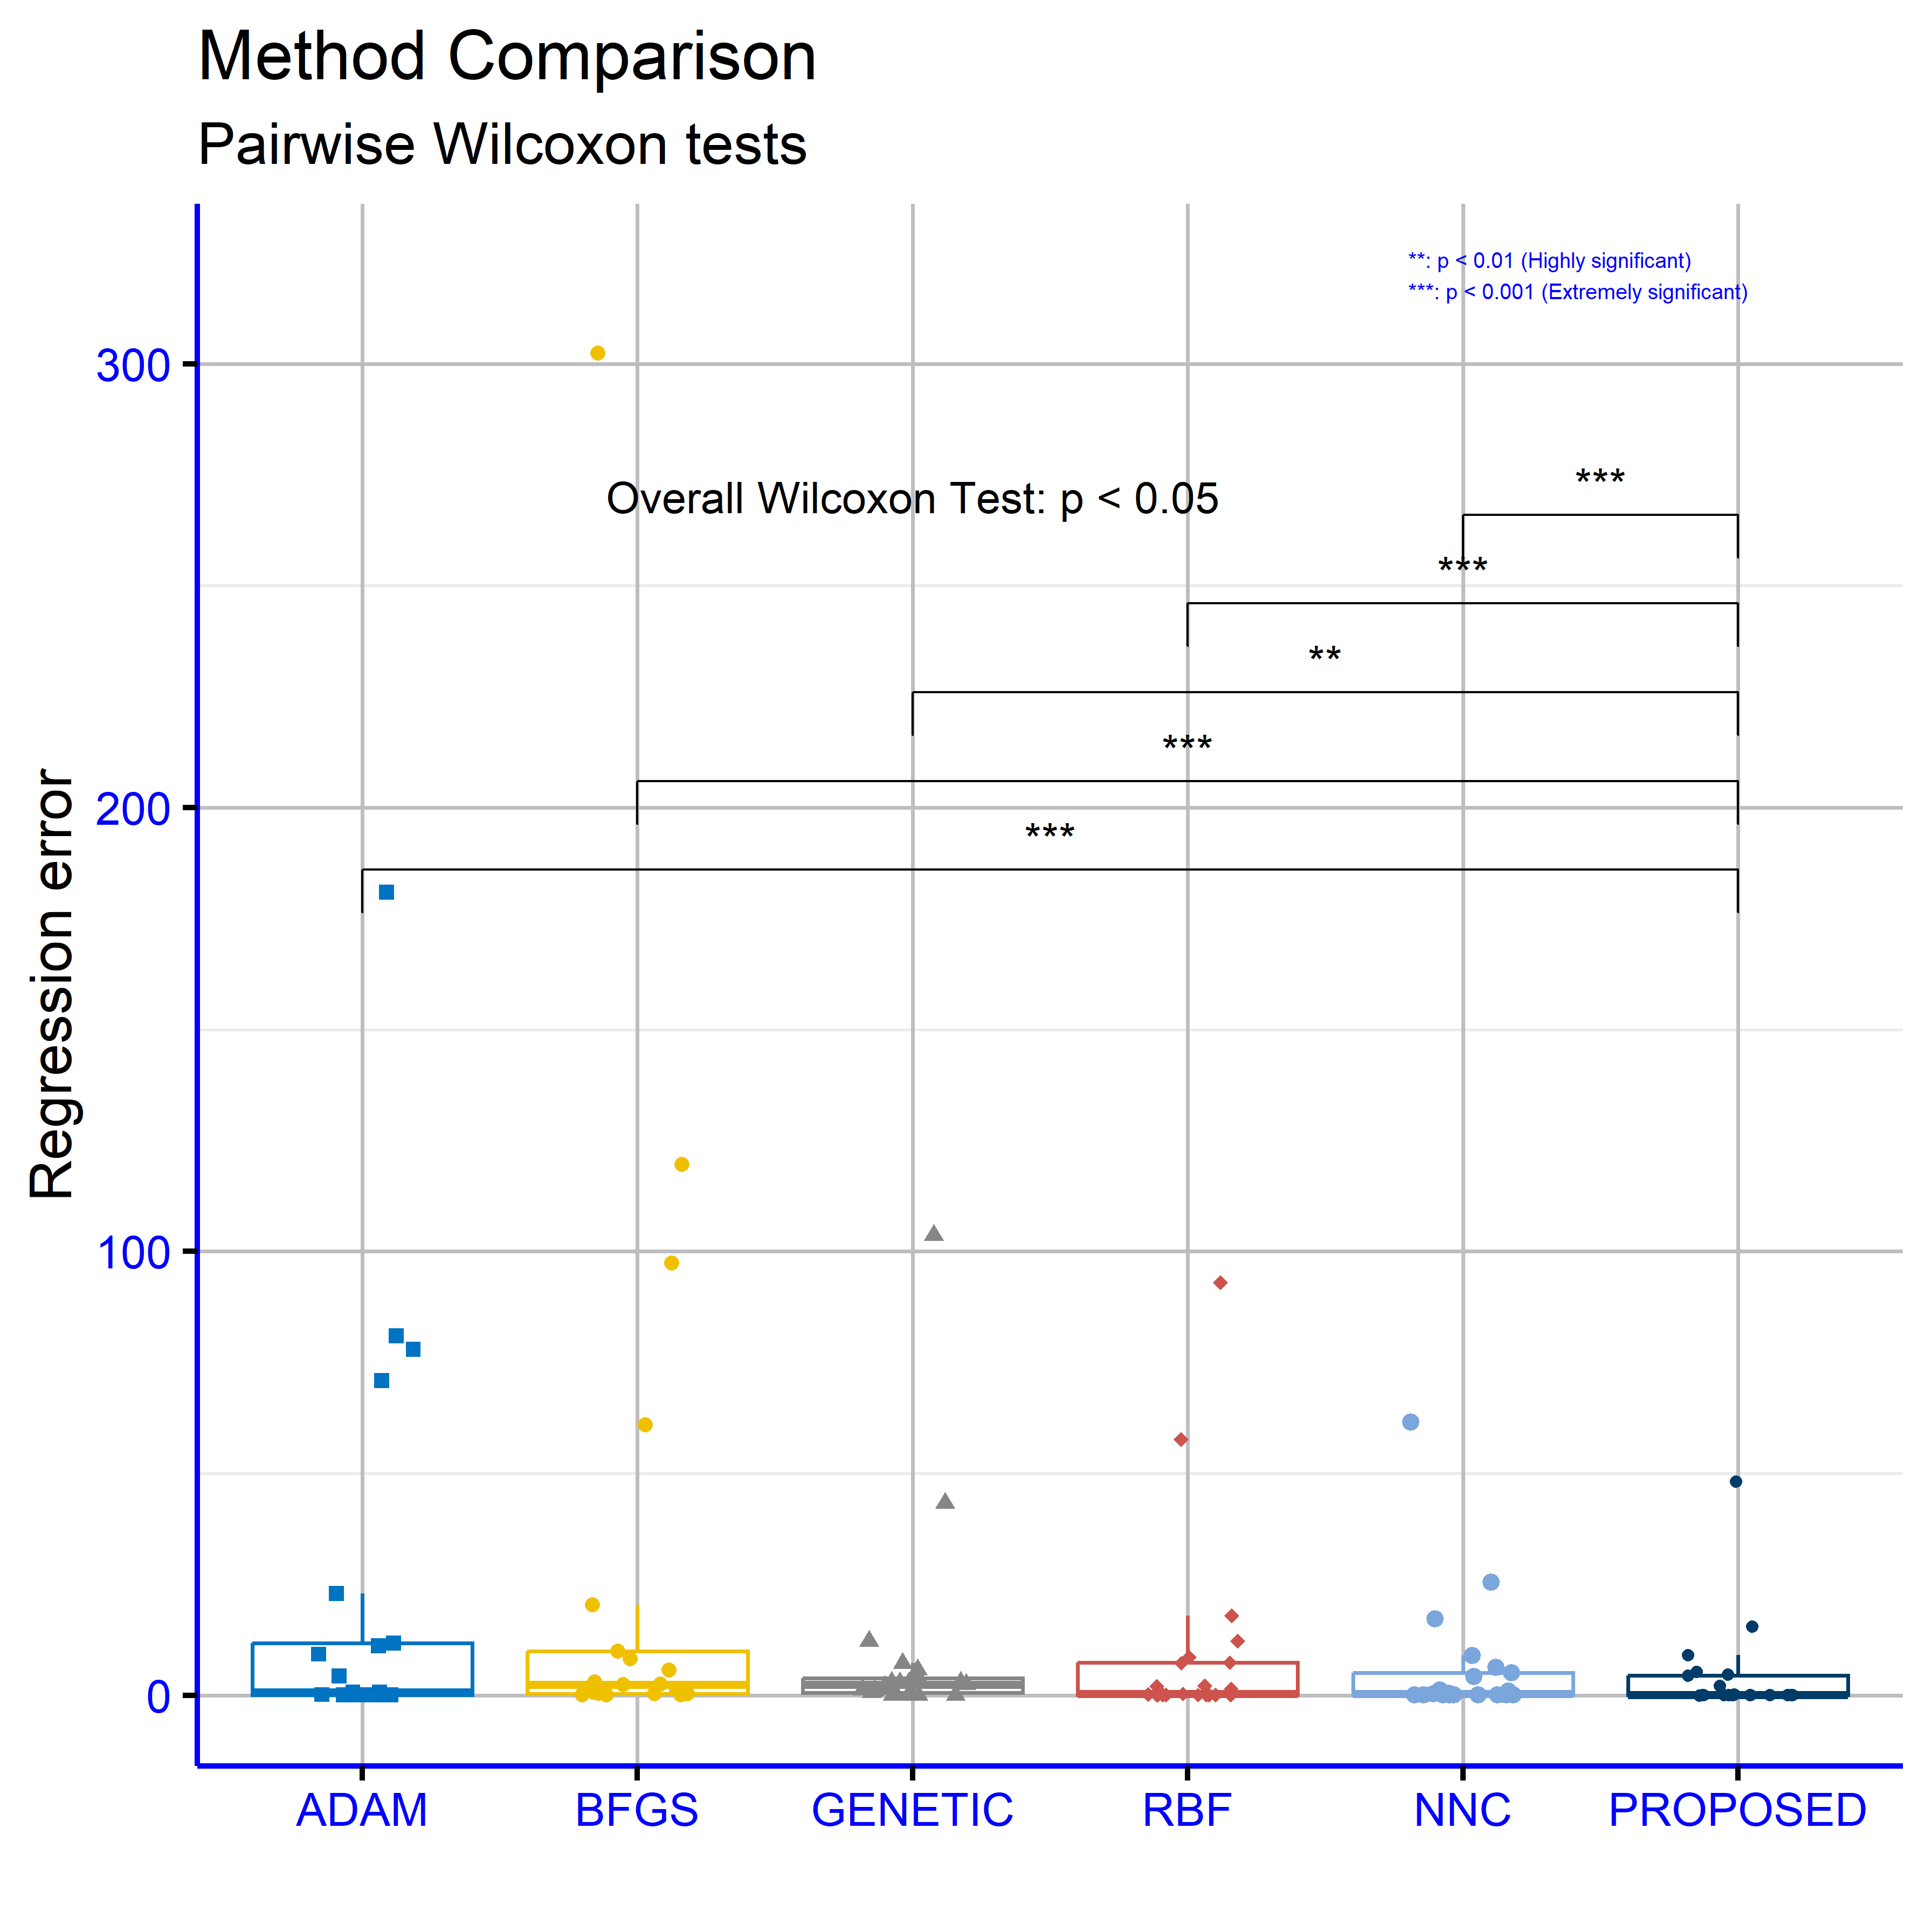
\includegraphics[scale=0.5]{new2}
\par\end{centering}
\caption{Statistical comparison between the used methods for the regression
datasets.\label{fig:statRegression}}

\end{figure}

Another experiment was conducted where the parameter $N_{K}$ was
altered in the range $[5,\ldots,50]$ and the results for the regression
datasets are depicted in Figure \ref{fig:nkExpers}.

\begin{figure}[H]
\begin{centering}
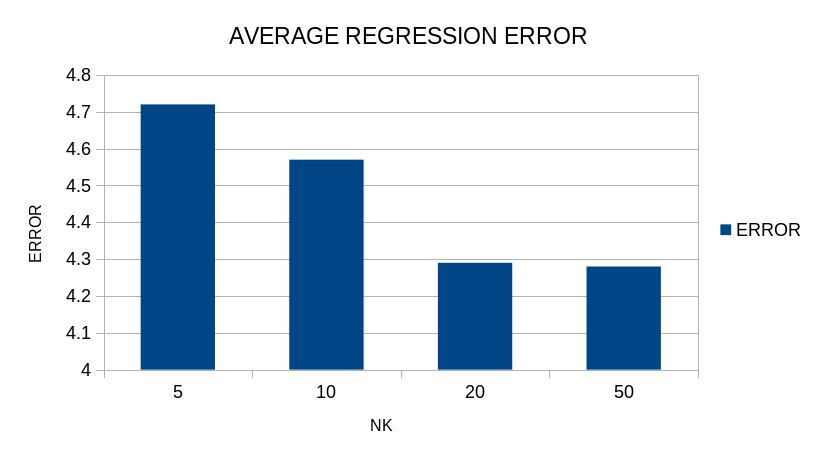
\includegraphics[scale=0.5]{nk_exper}
\par\end{centering}
\caption{Average regression error for the regression datasets and the proposed
method using a variety of values for the parameter $N_{K}$.\label{fig:nkExpers}}

\end{figure}
Additionally a series of experiments was conducted where the parameter
$N_{I}$ was changed from 10 to 40 and the results are graphically
presented in Figure \ref{fig:expersNI}.

\begin{figure}[H]
\begin{centering}
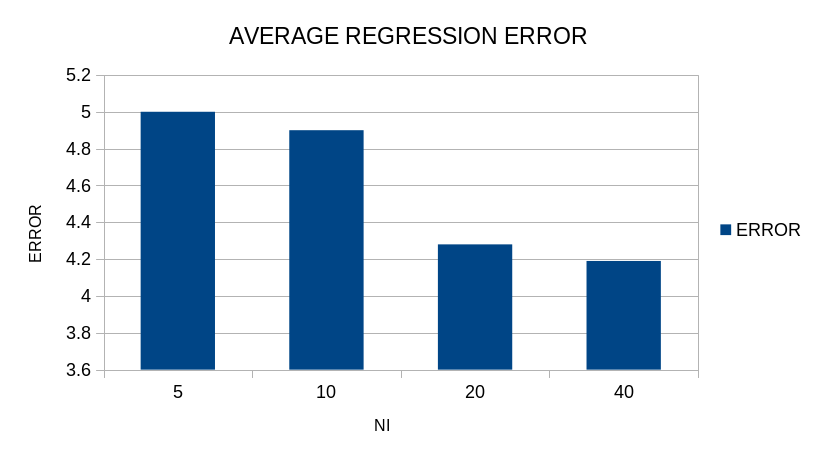
\includegraphics[scale=0.5]{ni_exper}
\par\end{centering}
\caption{Experimental results for the regression datasets and the proposed
method using a variety of values for the parameter $N_{I}$.\label{fig:expersNI}}

\end{figure}
Experimental measurements show that as the parameter $N_{I}$ increases,
the regression error decreases, indicating that higher values of $N_{I}$
contribute to improved model performance in regression tasks. Similarly,
increasing the parameter $N_{K}$ also results in a reduction in regression
error. This relationship highlights the importance of $N_{I}$ and
$N_{K}$ in optimizing the model's accuracy, possibly by influencing
the complexity or capacity of the neural network. These findings underscore
the significance of tuning $N_{I}$ and $N_{K}$ to achieve optimal
performance in regression applications.

\section{Conclusions\label{sec:Conclusions}}

The article presents a method for constructing artificial neural networks
by integrating Grammatical Evolution (GE) with a modified Genetic
Algorithm (GA) to improve generalization properties and reduce overfitting.
The method proves to be effective in designing neural network architectures
and optimizing their parameters. The modified genetic algorithm avoids
local minima during training and addresses overfitting by applying
penalty factors to the fitness function, ensuring better generalization
to unseen data. The method was evaluated on a variety of classification
and regression datasets from diverse fields, including physics, chemistry,
medicine, and economics. Comparative results indicate that the proposed
method achieves lower error rates on average compared to traditional
optimization and machine learning techniques, highlighting its stability
and adaptability. The results, analyzed through statistical metrics
such as p-values, provide strong evidence of the method’s superiority
over competing models in both classification and regression tasks.
A key innovation of the method is the combination of dynamic architecture
generation and parameter optimization within a unified framework.
This approach not only enhances performance but also reduces the computational
complexity associated with manually designing neural networks. Additionally,
the use of constraint techniques in the genetic algorithm ensures
the preservation of the neural network structure while enabling controlled
optimization of parameters. Future explorations could focus on testing
the method on larger and more complex datasets, such as those encountered
in image recognition, natural language processing, and genomics, to
evaluate its scalability and effectiveness in real-world applications.
Furthermore, the integration of other global optimization methods,
such as Particle Swarm Optimization, Simulated Annealing, or Differential
Evolution, could be considered to further enhance the algorithm’s
robustness and convergence speed. Concurrently, the inclusion of regularization
techniques, such as dropout or batch normalization, could improve
the method’s generalization capabilities even further. Reducing computational
cost is another important area of investigation, and the method could
be adapted to leverage parallel computing architectures, such as GPUs
or distributed systems, making it feasible for training on large datasets
or for real-time applications. Finally, customizing the grammar used
in Grammatical Evolution based on the specific characteristics of
individual fields could improve the method’s performance in specialized
tasks, such as time-series forecasting or anomaly detection in cybersecurity.

\vspace{6pt}


\authorcontributions{V.C. and I.G.T. conducted the experiments, employing several datasets
and provided the comparative experiments. D.T. and V.C. performed
the statistical analysis and prepared the manuscript. All authors
have read and agreed to the published version of the manuscript.}

\funding{This research received no external funding.}

\institutionalreview{Not applicable.}

\institutionalreview{Not applicable.}

\institutionalreview{Not applicable.}

\acknowledgments{This research has been financed by the European Union : Next Generation
EU through the Program Greece 2.0 National Recovery and Resilience
Plan , under the call RESEARCH -- CREATE -- INNOVATE, project name
“iCREW: Intelligent small craft simulator for advanced crew training
using Virtual Reality techniques\textquotedbl{} (project code:TAEDK-06195).}

\conflictsofinterest{The authors declare no conflicts of interest.}

\begin{adjustwidth}{-\extralength}{0cm}{}

\reftitle{References}
\begin{thebibliography}{99}
\bibitem{nn1}Abiodun, O. I., Jantan, A., Omolara, A. E., Dada, K.
V., Mohamed, N. A., \& Arshad, H. (2018). State-of-the-art in artificial
neural network applications: A survey. Heliyon, 4(11).

\bibitem{nn2}Suryadevara, S., \& Yanamala, A. K. Y. (2021). A Comprehensive
Overview of Artificial Neural Networks: Evolution, Architectures,
and Applications. Revista de Inteligencia Artificial en Medicina,
12(1), 51-76.

\bibitem{nn_image}M. Egmont-Petersen, D. de Ridder, H. Handels, Image
processing with neural networks---a review, Pattern Recognition \textbf{35},
pp. 2279-2301, 2002.

\bibitem{nn_timeseries}G.Peter Zhang, Time series forecasting using
a hybrid ARIMA and neural network model, Neurocomputing \textbf{50},
pp. 159-175, 2003.

\bibitem{nn_credit}Z. Huang, H. Chen, C.-Jung Hsu, W.-Hwa Chen, S.
Wu, Credit rating analysis with support vector machines and neural
networks: a market comparative study, Decision Support Systems \textbf{37},
pp. 543-558, 2004.

\bibitem{nnphysics1}P. Baldi, K. Cranmer, T. Faucett et al, Parameterized
neural networks for high-energy physics, Eur. Phys. J. C \textbf{76},
2016.

\bibitem{nnphysics2}Baldi, P., Cranmer, K., Faucett, T., Sadowski,
P., \& Whiteson, D. (2016). Parameterized neural networks for high-energy
physics. The European Physical Journal C, 76(5), 1-7.

\bibitem{bpnn1}Vora, K., \& Yagnik, S. (2014). A survey on backpropagation
algorithms for feedforward neural networks. International Journal
of Engineering Development and Research, 1(3), 193-197.

\bibitem{bpnn2}K. Vora, S. Yagnik, A survey on backpropagation algorithms
for feedforward neural networks, International Journal of Engineering
Development and Research \textbf{1}, pp. 193-197, 2014.

\bibitem{rpropnn-1}Pajchrowski, T., Zawirski, K., \& Nowopolski,
K. (2014). Neural speed controller trained online by means of modified
RPROP algorithm. IEEE transactions on industrial informatics, 11(2),
560-568.

\bibitem{rpropnn-2}Hermanto, R. P. S., \& Nugroho, A. (2018). Waiting-time
estimation in bank customer queues using RPROP neural networks. Procedia
Computer Science, 135, 35-42.

\bibitem{nn_adam}D. P. Kingma, J. L. Ba, ADAM: a method for stochastic
optimization, in: Proceedings of the 3rd International Conference
on Learning Representations (ICLR 2015), pp. 1--15, 2015.

\bibitem{geneticnn1}Reynolds, J., Rezgui, Y., Kwan, A., \& Piriou,
S. (2018). A zone-level, building energy optimisation combining an
artificial neural network, a genetic algorithm, and model predictive
control. Energy, 151, 729-739.

\bibitem{psonn}Das, G., Pattnaik, P. K., \& Padhy, S. K. (2014).
Artificial neural network trained by particle swarm optimization for
non-linear channel equalization. Expert Systems with Applications,
41(7), 3491-3496.

\bibitem{nn_siman}Sexton, R. S., Dorsey, R. E., \& Johnson, J. D.
(1999). Beyond backpropagation: using simulated annealing for training
neural networks. Journal of Organizational and End User Computing
(JOEUC), 11(3), 3-10.

\bibitem{weight_de1}Wang, L., Zeng, Y., \& Chen, T. (2015). Back
propagation neural network with adaptive differential evolution algorithm
for time series forecasting. Expert Systems with Applications, 42(2),
855-863.

\bibitem{nn_abc}Karaboga, D., \& Akay, B. (2007, June). Artificial
bee colony (ABC) algorithm on training artificial neural networks.
In 2007 IEEE 15th Signal Processing and Communications Applications
(pp. 1-4). IEEE.

\bibitem{tabunn}R.S. Sexton, B. Alidaee, R.E. Dorsey, J.D. Johnson,
Global optimization for artificial neural networks: A tabu search
application. European Journal of Operational Research \textbf{106},
pp. 570-584, 1998.

\bibitem{nn_hybrid}J.-R. Zhang, J. Zhang, T.-M. Lok, M.R. Lyu, A
hybrid particle swarm optimization--back-propagation algorithm for
feedforward neural network training, Applied Mathematics and Computation
\textbf{185}, pp. 1026-1037, 2007.

\bibitem{nn_cascade}G. Zhao, T. Wang, Y. Jin, C. Lang, Y. Li, H.
Ling, The Cascaded Forward algorithm for neural network training,
Pattern Recognition \textbf{161}, 111292, 2025.

\bibitem{nn_gpu1}K-Su Oh, K. Jung, GPU implementation of neural networks,
Pattern Recognition \textbf{37}, pp. 1311-1314, 2004.

\bibitem{nn_gpu2}M. Zhang, K. Hibi, J. Inoue, GPU-accelerated artificial
neural network potential for molecular dynamics simulation, Computer
Physics Communications \textbf{285}, 108655, 2023. 

\bibitem{nnsharing1}S.J. Nowlan and G.E. Hinton, Simplifying neural
networks by soft weight sharing, Neural Computation 4, pp. 473-493,
1992.

\bibitem{nnsharing2}Nowlan, S. J., \& Hinton, G. E. (2018). Simplifying
neural networks by soft weight sharing. In The mathematics of generalization
(pp. 373-394). CRC Press.

\bibitem{nnprunning1}S.J. Hanson and L.Y. Pratt, Comparing biases
for minimal network construction with back propagation, In D.S. Touretzky
(Ed.), Advances in Neural Information Processing Systems, Volume 1,
pp. 177-185, San Mateo, CA: Morgan Kaufmann, 1989.

\bibitem{nnprunning2}M. Augasta and T. Kathirvalavakumar, Pruning
algorithms of neural networks --- a comparative study, Central European
Journal of Computer Science, 2003.

\bibitem{nnearly1}Lutz Prechelt, Automatic early stopping using cross
validation: quantifying the criteria, Neural Networks \textbf{11},
pp. 761-767, 1998.

\bibitem{nnearly2}X. Wu and J. Liu, A New Early Stopping Algorithm
for Improving Neural Network Generalization, 2009 Second International
Conference on Intelligent Computation Technology and Automation, Changsha,
Hunan, 2009, pp. 15-18.

\bibitem{nndecay1}N. K. Treadgold and T. D. Gedeon, Simulated annealing
and weight decay in adaptive learning: the SARPROP algorithm,IEEE
Transactions on Neural Networks \textbf{9}, pp. 662-668, 1998.

\bibitem{nndecay2}M. Carvalho and T. B. Ludermir, Particle Swarm
Optimization of Feed-Forward Neural Networks with Weight Decay, 2006
Sixth International Conference on Hybrid Intelligent Systems (HIS'06),
Rio de Janeiro, Brazil, 2006, pp. 5-5.

\bibitem{nn_arch1}J. Arifovic, R. Gençay, Using genetic algorithms
to select architecture of a feedforward artificial neural network,
Physica A: Statistical Mechanics and its Applications \textbf{289},
pp. 574-594, 2001.

\bibitem{nn_arch2}P.G. Benardos, G.C. Vosniakos, Optimizing feedforward
artificial neural network architecture, Engineering Applications of
Artificial Intelligence \textbf{20}, pp. 365-382, 2007.

\bibitem{nn_arch3}B.A. Garro, R.A. Vázquez, Designing Artificial
Neural Networks Using Particle Swarm Optimization Algorithms, Computational
Intelligence and Neuroscience, 369298, 2015. 

\bibitem{ge1}M. O’Neill, C. Ryan, Grammatical evolution, IEEE Trans.
Evol. Comput. \textbf{5,}pp. 349--358, 2001.

\bibitem{nnc}I.G. Tsoulos, D. Gavrilis, E. Glavas, Neural network
construction and training using grammatical evolution, Neurocomputing
\textbf{72}, pp. 269-277, 2008.

\bibitem{nnc_amide1}G.V. Papamokos, I.G. Tsoulos, I.N. Demetropoulos,
E. Glavas, Location of amide I mode of vibration in computed data
utilizing constructed neural networks, Expert Systems with Applications
\textbf{36}, pp. 12210-12213, 2009.

\bibitem{nnc_de}I.G. Tsoulos, D. Gavrilis, E. Glavas, Solving differential
equations with constructed neural networks, Neurocomputing \textbf{72},
pp. 2385-2391, 2009.

\bibitem{nnc_feas}I.G. Tsoulos, G. Mitsi, A. Stavrakoudis, S. Papapetropoulos,
Application of Machine Learning in a Parkinson's Disease Digital Biomarker
Dataset Using Neural Network Construction (NNC) Methodology Discriminates
Patient Motor Status, Frontiers in ICT 6, 10, 2019.

\bibitem{nnc_student}V. Christou, I.G. Tsoulos, V. Loupas, A.T. Tzallas,
C. Gogos, P.S. Karvelis, N. Antoniadis, E. Glavas, N. Giannakeas,
Performance and early drop prediction for higher education students
using machine learning, Expert Systems with Applications \textbf{225},
120079, 2023.

\bibitem{nnc_autism}E.I. Toki, J. Pange, G. Tatsis, K. Plachouras,
I.G. Tsoulos, Utilizing Constructed Neural Networks for Autism Screening,
Applied Sciences \textbf{14}, 3053, 2024.

\bibitem{bnf1}J. W. Backus. The Syntax and Semantics of the Proposed
International Algebraic Language of the Zurich ACM-GAMM Conference.
Proceedings of the International Conference on Information Processing,
UNESCO, 1959, pp.125-132.

\bibitem{ge_program1}C. Ryan, J. Collins, M. O’Neill, Grammatical
evolution: Evolving programs for an arbitrary language. In: Banzhaf,
W., Poli, R., Schoenauer, M., Fogarty, T.C. (eds) Genetic Programming.
EuroGP 1998. Lecture Notes in Computer Science, vol 1391. Springer,
Berlin, Heidelberg, 1998.

\bibitem{ge_program2}M. O’Neill, M., C. Ryan, Evolving Multi-line
Compilable C Programs. In: Poli, R., Nordin, P., Langdon, W.B., Fogarty,
T.C. (eds) Genetic Programming. EuroGP 1999. Lecture Notes in Computer
Science, vol 1598. Springer, Berlin, Heidelberg, 1999.

\bibitem{ge_music}A.O. Puente, R. S. Alfonso, M. A. Moreno, Automatic
composition of music by means of grammatical evolution, In: APL '02:
Proceedings of the 2002 conference on APL: array processing languages:
lore, problems, and applications July 2002 Pages 148--155. 

\bibitem{ge_pacman}E. Galván-López, J.M. Swafford, M. O’Neill, A.
Brabazon, Evolving a Ms. PacMan Controller Using Grammatical Evolution.
In: , et al. Applications of Evolutionary Computation. EvoApplications
2010. Lecture Notes in Computer Science, vol 6024. Springer, Berlin,
Heidelberg, 2010.

\bibitem{ge_supermario}N. Shaker, M. Nicolau, G. N. Yannakakis, J.
Togelius, M. O'Neill, Evolving levels for Super Mario Bros using grammatical
evolution, 2012 IEEE Conference on Computational Intelligence and
Games (CIG), 2012, pp. 304-31.

\bibitem{ge_energy}D. Martínez-Rodríguez, J. M. Colmenar, J. I. Hidalgo,
R.J. Villanueva Micó, S. Salcedo-Sanz, Particle swarm grammatical
evolution for energy demand estimation, Energy Science and Engineering
\textbf{8}, pp. 1068-1079, 2020.

\bibitem{ge_crypt}C. Ryan, M. Kshirsagar, G. Vaidya, G. et al. Design
of a cryptographically secure pseudo random number generator with
grammatical evolution. Sci Rep \textbf{12}, 8602, 2022.

\bibitem{ge_trading}C. Martín, D. Quintana, P. Isasi, Grammatical
Evolution-based ensembles for algorithmic trading, Applied Soft Computing
\textbf{84}, 105713, 2019.

\bibitem{nnt_bound}Anastasopoulos, N., Tsoulos, I.G., Karvounis,
E. et al. Locate the Bounding Box of Neural Networks with Intervals.
Neural Process Lett 52, 2241--2251 (2020). 

\bibitem[(1989)]{uci} M. Kelly, R. Longjohn, K. Nottingham, The UCI
Machine Learning Repository, https://archive.ics.uci.edu.

\bibitem{Keel}J. Alcalá-Fdez, A. Fernandez, J. Luengo, J. Derrac,
S. García, L. Sánchez, F. Herrera. KEEL Data-Mining Software Tool:
Data Set Repository, Integration of Algorithms and Experimental Analysis
Framework. Journal of Multiple-Valued Logic and Soft Computing 17,
pp. 255-287, 2011.

\bibitem{appendicitis}Weiss, Sholom M. and Kulikowski, Casimir A.,
Computer Systems That Learn: Classification and Prediction Methods
from Statistics, Neural Nets, Machine Learning, and Expert Systems,
Morgan Kaufmann Publishers Inc, 1991.

\bibitem[Tzimourta(2018)]{alcohol}Tzimourta, K.D.; Tsoulos, I.; Bilero,
I.T.; Tzallas, A.T.; Tsipouras, M.G.; Giannakeas, N. Direct Assessment
of Alcohol Consumption in Mental State Using Brain Computer Interfaces
and Grammatical Evolution. Inventions 2018, 3, 51.

\bibitem[Quinlan(2018)]{australian}J.R. Quinlan, Simplifying Decision
Trees. International Journal of Man-Machine Studies \textbf{27}, pp.
221-234, 1987. 

\bibitem{balance}T. Shultz, D. Mareschal, W. Schmidt, Modeling Cognitive
Development on Balance Scale Phenomena, Machine Learning \textbf{16},
pp. 59-88, 1994.

\bibitem[(2004)]{cleveland1}Z.H. Zhou,Y. Jiang, NeC4.5: neural ensemble
based C4.5,\textquotedbl{} in IEEE Transactions on Knowledge and Data
Engineering \textbf{16}, pp. 770-773, 2004.

\bibitem{cleveland2}R. Setiono , W.K. Leow, FERNN: An Algorithm for
Fast Extraction of Rules from Neural Networks, Applied Intelligence
\textbf{12}, pp. 15-25, 2000.

\bibitem[(1998)]{dermatology}G. Demiroz, H.A. Govenir, N. Ilter,
Learning Differential Diagnosis of Eryhemato-Squamous Diseases using
Voting Feature Intervals, Artificial Intelligence in Medicine. \textbf{13},
pp. 147--165, 1998.

\bibitem[(1996)]{ecoli}P. Horton, K.Nakai, A Probabilistic Classification
System for Predicting the Cellular Localization Sites of Proteins,
In: Proceedings of International Conference on Intelligent Systems
for Molecular Biology \textbf{4}, pp. 109-15, 1996.

\bibitem[(1977)]{hayes-roth}B. Hayes-Roth, B., F. Hayes-Roth. Concept
learning and the recognition and classification of exemplars. Journal
of Verbal Learning and Verbal Behavior \textbf{16}, pp. 321-338, 1977.

\bibitem[(1997)]{heart}I. Kononenko, E. Šimec, M. Robnik-Šikonja,
Overcoming the Myopia of Inductive Learning Algorithms with RELIEFF,
Applied Intelligence \textbf{7}, pp. 39--55, 1997

\bibitem[(2002)]{housevotes}R.M. French, N. Chater, Using noise to
compute error surfaces in connectionist networks: a novel means of
reducing catastrophic forgetting, Neural Comput. \textbf{14}, pp.
1755-1769, 2002.

\bibitem[(2004)]{ion1}J.G. Dy , C.E. Brodley, Feature Selection for
Unsupervised Learning, The Journal of Machine Learning Research \textbf{5},
pp 845--889, 2004.

\bibitem{ion2}S. J. Perantonis, V. Virvilis, Input Feature Extraction
for Multilayered Perceptrons Using Supervised Principal Component
Analysis, Neural Processing Letters \textbf{10}, pp 243--252, 1999.

\bibitem[(2002)]{liver} J. Garcke, M. Griebel, Classification with
sparse grids using simplicial basis functions, Intell. Data Anal.
\textbf{6}, pp. 483-502, 2002.

\bibitem{liver1}J. Mcdermott, R.S. Forsyth, Diagnosing a disorder
in a classification benchmark, Pattern Recognition Letters \textbf{73},
pp. 41-43, 2016.

\bibitem[(2002)]{lymography}G. Cestnik, I. Konenenko, I. Bratko,
Assistant-86: A Knowledge-Elicitation Tool for Sophisticated Users.
In: Bratko, I. and Lavrac, N., Eds., Progress in Machine Learning,
Sigma Press, Wilmslow, pp. 31-45, 1987. 

\bibitem[(2007)]{mammographic}M. Elter, R. Schulz-Wendtland, T. Wittenberg,
The prediction of breast cancer biopsy outcomes using two CAD approaches
that both emphasize an intelligible decision process, Med Phys. \textbf{34},
pp. 4164-72, 2007.

\bibitem[(2007)]{parkinsons1}M.A. Little, P.E. McSharry, S.J Roberts
et al, Exploiting Nonlinear Recurrence and Fractal Scaling Properties
for Voice Disorder Detection. BioMed Eng OnLine \textbf{6}, 23, 2007.

\bibitem{parkinsons2}M.A. Little, P.E. McSharry, E.J. Hunter, J.
Spielman, L.O. Ramig, Suitability of dysphonia measurements for telemonitoring
of Parkinson's disease. IEEE Trans Biomed Eng. \textbf{56}, pp. 1015-1022,
2009.

\bibitem[(2007)]{pima}J.W. Smith, J.E. Everhart, W.C. Dickson, W.C.
Knowler, R.S. Johannes, Using the ADAP learning algorithm to forecast
the onset of diabetes mellitus, In: Proceedings of the Symposium on
Computer Applications and Medical Care IEEE Computer Society Press,
pp.261-265, 1988.

\bibitem[(2007)]{popfailures}D.D. Lucas, R. Klein, J. Tannahill,
D. Ivanova, S. Brandon, D. Domyancic, Y. Zhang, Failure analysis of
parameter-induced simulation crashes in climate models, Geoscientific
Model Development \textbf{6}, pp. 1157-1171, 2013.

\bibitem[(2007)]{regions2}N. Giannakeas, M.G. Tsipouras, A.T. Tzallas,
K. Kyriakidi, Z.E. Tsianou, P. Manousou, A. Hall, E.C. Karvounis,
V. Tsianos, E. Tsianos, A clustering based method for collagen proportional
area extraction in liver biopsy images (2015) Proceedings of the Annual
International Conference of the IEEE Engineering in Medicine and Biology
Society, EMBS, 2015-November, art. no. 7319047, pp. 3097-3100. 

\bibitem[(2007)]{saheart}T. Hastie, R. Tibshirani, Non-parametric
logistic and proportional odds regression, JRSS-C (Applied Statistics)
\textbf{36}, pp. 260--276, 1987.

\bibitem{segment}M. Dash, H. Liu, P. Scheuermann, K. L. Tan, Fast
hierarchical clustering and its validation, Data \& Knowledge Engineering
\textbf{44}, pp 109--138, 2003.

\bibitem[(2007)]{student}P. Cortez, A. M. Gonçalves Silva, Using
data mining to predict secondary school student performance, In Proceedings
of 5th FUture BUsiness TEChnology Conference (FUBUTEC 2008) (pp. 5--12).
EUROSIS-ETI, 2008.

\bibitem[(2007)]{transfusion}I-Cheng Yeh, King-Jang Yang, Tao-Ming
Ting, Knowledge discovery on RFM model using Bernoulli sequence, Expert
Systems with Applications \textbf{36}, pp. 5866-5871, 2009.

\bibitem[(2007)]{wdbc1}Jeyasingh, S., \& Veluchamy, M. (2017). Modified
bat algorithm for feature selection with the Wisconsin diagnosis breast
cancer (WDBC) dataset. Asian Pacific journal of cancer prevention:
APJCP, 18(5), 1257.

\bibitem[(2007)]{wdbc2}Alshayeji, M. H., Ellethy, H., \& Gupta, R.
(2022). Computer-aided detection of breast cancer on the Wisconsin
dataset: An artificial neural networks approach. Biomedical signal
processing and control, 71, 103141.

\bibitem[(2007)]{wine1}M. Raymer, T.E. Doom, L.A. Kuhn, W.F. Punch,
Knowledge discovery in medical and biological datasets using a hybrid
Bayes classifier/evolutionary algorithm. IEEE transactions on systems,
man, and cybernetics. Part B, Cybernetics : a publication of the IEEE
Systems, Man, and Cybernetics Society, \textbf{33} , pp. 802-813,
2003.

\bibitem{wine2}P. Zhong, M. Fukushima, Regularized nonsmooth Newton
method for multi-class support vector machines, Optimization Methods
and Software \textbf{22}, pp. 225-236, 2007.

\bibitem[(2007)]{eeg1}R. G. Andrzejak, K. Lehnertz, F.Mormann, C.
Rieke, P. David, and C. E. Elger, “Indications of nonlinear deterministic
and finite-dimensional structures in time series of brain electrical
activity: dependence on recording region and brain state,” Physical
Review E, vol. 64, no. 6, Article ID 061907, 8 pages, 2001. 

\bibitem{eeg2}A. T. Tzallas, M. G. Tsipouras, and D. I. Fotiadis,
“Automatic Seizure Detection Based on Time-Frequency Analysis and
Artificial Neural Networks,” Computational Intelligence and Neuroscience,
vol. 2007, Article ID 80510, 13 pages, 2007. doi:10.1155/2007/80510

\bibitem[(2007)]{zoo}M. Koivisto, K. Sood, Exact Bayesian Structure
Discovery in Bayesian Networks, The Journal of Machine Learning Research\textbf{
5}, pp. 549--573, 2004.

\bibitem[(2007)]{abalone}Nash, W.J.; Sellers, T.L.; Talbot, S.R.;
Cawthor, A.J.; Ford, W.B. The Population Biology of Abalone (\_Haliotis\_
species) in Tasmania. I. Blacklip Abalone (\_H. rubra\_) from the
North Coast and Islands of Bass Strait, Sea Fisheries Division; Technical
Report No. 48; Department of Primary Industry and Fisheries, Tasmania:
Hobart, Australia, 1994; ISSN 1034-3288

\bibitem[(2007)]{airfoil}Brooks, T.F.; Pope, D.S.; Marcolini, A.M.
Airfoil Self-Noise and Prediction. Technical Report, NASA RP-1218.
July 1989. Available online: https://ntrs.nasa.gov/citations/19890016302
(accessed on 14 November 2024).

\bibitem[(2007)]{concrete}I.Cheng Yeh, Modeling of strength of high
performance concrete using artificial neural networks, Cement and
Concrete Research. \textbf{28}, pp. 1797-1808, 1998. 

\bibitem{friedman}Friedman, J. (1991): Multivariate Adaptative Regression
Splines. Annals of Statistics, 19:1, 1-{}-141. 

\bibitem[(2007)]{housing}D. Harrison and D.L. Rubinfeld, Hedonic
prices and the demand for clean ai, J. Environ. Economics \& Management
\textbf{5}, pp. 81-102, 1978.

\bibitem{powell}M.J.D Powell, A Tolerant Algorithm for Linearly Constrained
Optimization Calculations, Mathematical Programming \textbf{45}, pp.
547-566, 1989. 

\bibitem[(1991)]{rbf1}J. Park and I. W. Sandberg, Universal Approximation
Using Radial-Basis-Function Networks, Neural Computation \textbf{3},
pp. 246-257, 1991.

\bibitem{rbf2}G.A. Montazer, D. Giveki, M. Karami, H. Rastegar, Radial
basis function neural networks: A review. Comput. Rev. J \textbf{1},
pp. 52-74, 2018.

\end{thebibliography}

\end{adjustwidth}{}
\end{document}
